\documentclass[]{book}
\usepackage{lmodern}
\usepackage{amssymb,amsmath}
\usepackage{ifxetex,ifluatex}
\usepackage{fixltx2e} % provides \textsubscript
\ifnum 0\ifxetex 1\fi\ifluatex 1\fi=0 % if pdftex
  \usepackage[T1]{fontenc}
  \usepackage[utf8]{inputenc}
\else % if luatex or xelatex
  \ifxetex
    \usepackage{mathspec}
  \else
    \usepackage{fontspec}
  \fi
  \defaultfontfeatures{Ligatures=TeX,Scale=MatchLowercase}
\fi
% use upquote if available, for straight quotes in verbatim environments
\IfFileExists{upquote.sty}{\usepackage{upquote}}{}
% use microtype if available
\IfFileExists{microtype.sty}{%
\usepackage{microtype}
\UseMicrotypeSet[protrusion]{basicmath} % disable protrusion for tt fonts
}{}
\usepackage{hyperref}
\hypersetup{unicode=true,
            pdftitle={Tölfræði 3 fyrir BS nema í Sálfræði (útgáfa 0.1 haust 2019)},
            pdfauthor={Anton Örn Karlsson},
            pdfborder={0 0 0},
            breaklinks=true}
\urlstyle{same}  % don't use monospace font for urls
\usepackage{natbib}
\bibliographystyle{apalike}
\usepackage{color}
\usepackage{fancyvrb}
\newcommand{\VerbBar}{|}
\newcommand{\VERB}{\Verb[commandchars=\\\{\}]}
\DefineVerbatimEnvironment{Highlighting}{Verbatim}{commandchars=\\\{\}}
% Add ',fontsize=\small' for more characters per line
\usepackage{framed}
\definecolor{shadecolor}{RGB}{248,248,248}
\newenvironment{Shaded}{\begin{snugshade}}{\end{snugshade}}
\newcommand{\AlertTok}[1]{\textcolor[rgb]{0.94,0.16,0.16}{#1}}
\newcommand{\AnnotationTok}[1]{\textcolor[rgb]{0.56,0.35,0.01}{\textbf{\textit{#1}}}}
\newcommand{\AttributeTok}[1]{\textcolor[rgb]{0.77,0.63,0.00}{#1}}
\newcommand{\BaseNTok}[1]{\textcolor[rgb]{0.00,0.00,0.81}{#1}}
\newcommand{\BuiltInTok}[1]{#1}
\newcommand{\CharTok}[1]{\textcolor[rgb]{0.31,0.60,0.02}{#1}}
\newcommand{\CommentTok}[1]{\textcolor[rgb]{0.56,0.35,0.01}{\textit{#1}}}
\newcommand{\CommentVarTok}[1]{\textcolor[rgb]{0.56,0.35,0.01}{\textbf{\textit{#1}}}}
\newcommand{\ConstantTok}[1]{\textcolor[rgb]{0.00,0.00,0.00}{#1}}
\newcommand{\ControlFlowTok}[1]{\textcolor[rgb]{0.13,0.29,0.53}{\textbf{#1}}}
\newcommand{\DataTypeTok}[1]{\textcolor[rgb]{0.13,0.29,0.53}{#1}}
\newcommand{\DecValTok}[1]{\textcolor[rgb]{0.00,0.00,0.81}{#1}}
\newcommand{\DocumentationTok}[1]{\textcolor[rgb]{0.56,0.35,0.01}{\textbf{\textit{#1}}}}
\newcommand{\ErrorTok}[1]{\textcolor[rgb]{0.64,0.00,0.00}{\textbf{#1}}}
\newcommand{\ExtensionTok}[1]{#1}
\newcommand{\FloatTok}[1]{\textcolor[rgb]{0.00,0.00,0.81}{#1}}
\newcommand{\FunctionTok}[1]{\textcolor[rgb]{0.00,0.00,0.00}{#1}}
\newcommand{\ImportTok}[1]{#1}
\newcommand{\InformationTok}[1]{\textcolor[rgb]{0.56,0.35,0.01}{\textbf{\textit{#1}}}}
\newcommand{\KeywordTok}[1]{\textcolor[rgb]{0.13,0.29,0.53}{\textbf{#1}}}
\newcommand{\NormalTok}[1]{#1}
\newcommand{\OperatorTok}[1]{\textcolor[rgb]{0.81,0.36,0.00}{\textbf{#1}}}
\newcommand{\OtherTok}[1]{\textcolor[rgb]{0.56,0.35,0.01}{#1}}
\newcommand{\PreprocessorTok}[1]{\textcolor[rgb]{0.56,0.35,0.01}{\textit{#1}}}
\newcommand{\RegionMarkerTok}[1]{#1}
\newcommand{\SpecialCharTok}[1]{\textcolor[rgb]{0.00,0.00,0.00}{#1}}
\newcommand{\SpecialStringTok}[1]{\textcolor[rgb]{0.31,0.60,0.02}{#1}}
\newcommand{\StringTok}[1]{\textcolor[rgb]{0.31,0.60,0.02}{#1}}
\newcommand{\VariableTok}[1]{\textcolor[rgb]{0.00,0.00,0.00}{#1}}
\newcommand{\VerbatimStringTok}[1]{\textcolor[rgb]{0.31,0.60,0.02}{#1}}
\newcommand{\WarningTok}[1]{\textcolor[rgb]{0.56,0.35,0.01}{\textbf{\textit{#1}}}}
\usepackage{longtable,booktabs}
\usepackage{graphicx}
% grffile has become a legacy package: https://ctan.org/pkg/grffile
\IfFileExists{grffile.sty}{%
\usepackage{grffile}
}{}
\makeatletter
\def\maxwidth{\ifdim\Gin@nat@width>\linewidth\linewidth\else\Gin@nat@width\fi}
\def\maxheight{\ifdim\Gin@nat@height>\textheight\textheight\else\Gin@nat@height\fi}
\makeatother
% Scale images if necessary, so that they will not overflow the page
% margins by default, and it is still possible to overwrite the defaults
% using explicit options in \includegraphics[width, height, ...]{}
\setkeys{Gin}{width=\maxwidth,height=\maxheight,keepaspectratio}
\IfFileExists{parskip.sty}{%
\usepackage{parskip}
}{% else
\setlength{\parindent}{0pt}
\setlength{\parskip}{6pt plus 2pt minus 1pt}
}
\setlength{\emergencystretch}{3em}  % prevent overfull lines
\providecommand{\tightlist}{%
  \setlength{\itemsep}{0pt}\setlength{\parskip}{0pt}}
\setcounter{secnumdepth}{5}
% Redefines (sub)paragraphs to behave more like sections
\ifx\paragraph\undefined\else
\let\oldparagraph\paragraph
\renewcommand{\paragraph}[1]{\oldparagraph{#1}\mbox{}}
\fi
\ifx\subparagraph\undefined\else
\let\oldsubparagraph\subparagraph
\renewcommand{\subparagraph}[1]{\oldsubparagraph{#1}\mbox{}}
\fi

%%% Use protect on footnotes to avoid problems with footnotes in titles
\let\rmarkdownfootnote\footnote%
\def\footnote{\protect\rmarkdownfootnote}

%%% Change title format to be more compact
\usepackage{titling}

% Create subtitle command for use in maketitle
\providecommand{\subtitle}[1]{
  \posttitle{
    \begin{center}\large#1\end{center}
    }
}

\setlength{\droptitle}{-2em}

  \title{Tölfræði 3 fyrir BS nema í Sálfræði (útgáfa 0.1 haust 2019)}
    \pretitle{\vspace{\droptitle}\centering\huge}
  \posttitle{\par}
    \author{Anton Örn Karlsson}
    \preauthor{\centering\large\emph}
  \postauthor{\par}
      \predate{\centering\large\emph}
  \postdate{\par}
    \date{2019-11-24}

\usepackage{booktabs}

\begin{document}
\maketitle

{
\setcounter{tocdepth}{1}
\tableofcontents
}
\hypertarget{inngangur}{%
\chapter{Inngangur}\label{inngangur}}

Ritið sem hér fylgir á eftir er yfirlit yfir kennsluefni úr Tölfræði 3 fyrir BS nema í Sálfræði við Háskóla Íslands.

Í þessari fyrstu útgáfu er fjallað um aðhvarfsgreiningu hlutfalla og þáttagreiningu.

Vinsamlegast athugið að um er að ræða óyfirlesnar og óleiðréttar kennsluglósur sem byggðar eru á kennslubók námskeiðisins. \textbf{Villur kunna því að leynast í textanum!}

Allar athugasemdir og spurningar sendist á \href{mailto:anton.karlsson@hagstofa.is}{\nolinkurl{anton.karlsson@hagstofa.is}}

\hypertarget{auxf0fallsgreining-hlutfalla}{%
\chapter{Aðfallsgreining hlutfalla}\label{auxf0fallsgreining-hlutfalla}}

\hypertarget{logreg-inngangur}{%
\section{Inngangur}\label{logreg-inngangur}}

Byggir á línulegri aðfallsgreiningu. Nema þar vorum við að nota samfellda fylgibreytu og eina eða fleiri frumbreytur í líkani þar sem við erum að fjalla um sambandið þarna á milli.

Þegar við erum með fylgibreytu sem er flokkabreyta með tveimur möguleikum þá notum við annars konar tegund aðferðar til að kanna tengslin. Sú aðferð er nefnd aðfallsgreining hlutfalla eða logistic regression uppá ensku.

Mikilvægt er að fylgibreytan er sett upp sem tvíkosta breyta sem tekur aðeins gildin 0 og 1. Þá er einnig hægt að segja að 1 standi fyrir árangur og 0 standi fyrir að misheppnast. Ef við tökum meðaltal af breytu af þessu tagi þá fáum við hlutfall árangurs - þannig að meðaltal af tvíkostabreytu með gildin 0 og 1 gefur okkur alltaf hlutfall þeirra sem eru með 1 í gagnasafninu.

Ef um er að ræða gögn með óháða tvíkosta breytu þá er talað um tvíliða gögn (binomial setting). Það eru fjórar forsendur sem þarf að uppfylla í tilraun til að um sé að ræða binomial setting:
1) hver mæling fellur í einn tveggja flokka sem eru kallaðir success/failure
2) það er endanlegur fjöldi mælinga
3) allar mælingarnar eru óháðar
4) líkurnar á success eru þær sömu fyrir allar mælingarnar - jafnar

Ef tilraunin er með binomial setting, þá er handahófsbreytan X fjöldi successes binomial random breyta og líkindadreifing X er tvílhiða dreifingu (binomial distribution)

\hypertarget{duxe6mi-um-tvuxedkostabreytur}{%
\section{Dæmi um tvíkostabreytur}\label{duxe6mi-um-tvuxedkostabreytur}}

Sem dæmi um breytur sem eru tvíliða og nota má í aðfallsgreiningu hlutfalla eru:

\begin{itemize}
\tightlist
\item
  staðið eða fall í áfanga
\item
  hvort viðkomandi nái greiningarviðmiðum þunglyndis
\item
  mat á eigin heilsufari (til dæmis, endurkóðað úr fimm punkta kvarða í tvíkosta breytu)
\item
  hvort viðkomandi drekki kaffi eða ekki
\end{itemize}

\hypertarget{tvuxedliuxf0udreifing}{%
\section{Tvíliðudreifing}\label{tvuxedliuxf0udreifing}}

Tvíliðudreifing er dreifing á talningu breytunnar X (það er talning á tilvikum þar sem X er 1) undir tvíliðu setting með tvo stika: n og p.~n stendur fyrir fjölda mælinga og p eru líkurnar á árangri fyrir hverja einstaka mælingu. Möguleg gildi X eru heiltölur frá 0 til n og er skrifuð X is B(n,p).

\begin{figure}

{\centering 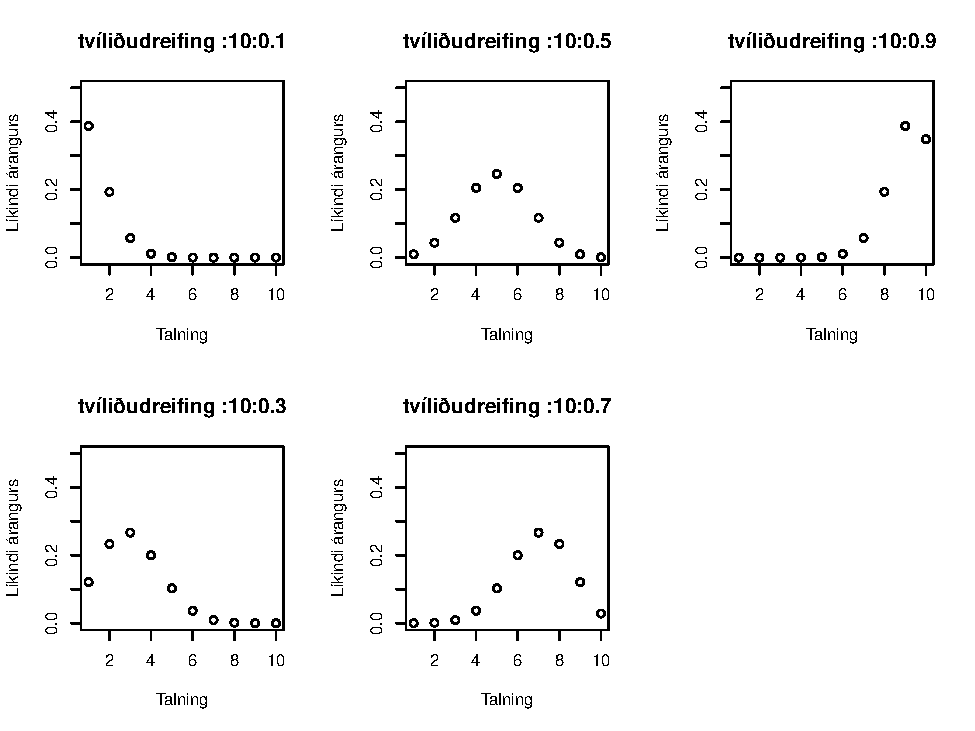
\includegraphics[width=0.8\linewidth]{timaglosur_files/figure-latex/binom-dist-1} 

}

\caption{Tvíliðudreifingar með mismunandi stikum}\label{fig:binom-dist}
\end{figure}

Á mynd \ref{fig:binom-dist} má sjá tvíliðudreifingu með mismunandi stikum. Í efri línunni fyrir miðju má sjá tvíliðudreifingu þar sem stikarnir eru 0.5 og 10 - sem merkir að úrtakið er af stærðinni 10 og líkurnar er 0.5. Þarna sjáum við að hæstu líkurnar eru við fimm - sem merkir að þar sem undirliggjandi líkurnar eru 0.5 þá eru hæstar líkur á að fá 5 árangursrík tilvik í úrtaki 10 tilvika. Til dæmis ef við köstum krónu 10 sinnum og við ætluðum að telja hversu oft landvætturinn birtist, þá myndum við búast við að eðlileg króna myndi fimm sinnum lenda á bergrisanum. En hins vegar sjáum við líka að það er eðlilegt að krónan myndi lenda fjórum sinnum eða sex sinnum á landvættinum þar sem líkurnar á þeim eru ekki langt frá líkunum á fimm sinnum. Með öðrum orðum, það væri ekki ólíklegt að kasta krónu tíu sinnum og í fjórum eða sex tilvikum myndum við fá bergrisann en samt væri um að ræða eðlilegan krónupening.

\hypertarget{hl-likur}{%
\section{Hlutfallslíkur}\label{hl-likur}}

\emph{p} er hlutfallið af hópnum sem er með gildið 1 á tiltekinni tvíkostabreytu (eða success). Ef við værum með handahófskennt úrtak af stærðinni \emph{n} úr þýði þá dreifist fjöldi þeirra sem er með gildið einn (eða success) miðað við binomial dreifingu með parametrunum \emph{n} og \emph{p}.

Hlutfallið er þá fjöldi þeirra sem eru með 1 á móti heildarfjölda í úrtakinu. Það merkjum við sem p-hatt þar sem um er að ræða mat á hlutfalli þýðisins á grundvelli úrtaksins.

Þegar við notum aðfallsgreiningu hlutfalla þá notum við hins vegar hlutfallslíkur í stað hlutfalla. Hlutfallslíkur er hlutfallið milli hinna tveggja mögulegu útkoma (það er, hlutfallið milli þeirra sem eru með gildið 1 og þeirra sem eru með gildið 0 á tvíkostabreytunni).

\(hl=\frac{\hat{p} }{1-\hat{p}}\)

Til dæmis gætum við tekið 1000 manna úrtak úr þjóðskrá og myndum spyrja alla hvort þeir hefðu kosið í síðustu kosningum. Í ljós kæmi að 700 þeirra hefðu kosið. Það merkir að hlutfallið er \(\hat{p}=\) 0.7 en hlutfallslíkurnar eru 2.33

Með því að námunda hlutfallslíkur þess að hafa kosið í síðustu kosningum má sjá að kjósendur eru um 2 á móti 1 - fyrir hverja 2 kjósendur var einn sem ekki kaus.

Annað dæmi gæti verið að draga spil af handahófi úr spilastokk. Ef við gerum það þá vitum við líkurnar á að draga spaða eru 13/52 eða 1/4 sem við getum einnig skrifað sem tugabrot 0.25. Hlutfallslíkurnar á því að draga spaða eru 0.33. Hins vegar eru hlutfallslíkurnar á að draga spil af öðrum lit 3 á móti 1.

\hypertarget{hlutfallsluxedkur-tveggja-huxf3pa}{%
\section{Hlutfallslíkur tveggja hópa}\label{hlutfallsluxedkur-tveggja-huxf3pa}}

Við höfum áður skoðað hvernig hægt er að bera saman tvö hlutföll í úrtaki, til dæmis hvort karlar eða konur séu líklegri til að nota Instagram. Í því tilviki skoðum við muninn á hlutfalli beggja hópa og reiknum öryggisbil utan um muninn. Ef öryggisbilið inniheldur ekki núll þá getum við ályktað sem svo að líklega sé um að ræða mun á instagram notkun í þýðinu.

Önnur leið til að meta hvort kyn tengist líkum þess að nota Instagram er að framkvæma aðfallsgreiningu hlutfalla. Það sem gerir hana enn árangursríkari sem aðferð til að kanna tengsl milli breyta er að hún tekur fleiri en eina frumbreytu. Ennfremur er aðfallsgreining hlutfalla, rétt eins og línuleg aðfallsgreining, sveigjanleg að því marki að hægt er að setja fram sveiglínusamband og samvirkni milli tveggja eða fleiri frumbreyta í líkaninu. A Aðfallsgreining hlufalla hentar hvort sem er fyrir samfelldar eða flokkaðar frumbreytur en fylgibreytan er alltaf tvíkosta og tekur gildin 0 og 1.

\hypertarget{af-hverju-ekki-auxf0-nota-luxednulega-auxf0fallsgreiningu}{%
\section{Af hverju ekki að nota línulega aðfallsgreiningu?}\label{af-hverju-ekki-auxf0-nota-luxednulega-auxf0fallsgreiningu}}

Tæknilega séð er hægt að nota línulega aðfallsgreiningu þegar fylgibreytan er tvíkosta en það getur hins vegar dregið dilk á eftir sér. Skoðum dæmi.

Í félagskönnun í Bandaríkjunum er spurt um sjónvarpsáhorf. Þar mætti til dæmis skoða að hvaða marki aldur tengist sjónvarpsháorfi. Í þessu tilviki ætlum við að skoða að hvaða marki aldur tengist því hvort fólk horfi á sjónvarp lengur en 6 klukkustundir á dag.

Samkvæmt gagnasafninu okkar horfa um 24\% Bandaríkjamanna í sex klukkustundir eða lengur á sjónvarpið á degi hverjum. Ef við setjum upp línulegt aðfallsgreiningarlíkan þá kemur hins vegar strax í ljós að það býr til spágildi sem geta ekki gengið upp þar sem þau lenda undir núlli - eru neikvæðar. Það má sjá á \ref{fig:two-models} þar sem rauða línan stendur fyrir spágildi línulega líkansins. Eins og sjá má verða spágildi þeirra sem eru 30 ára og yngri neikvæð, en það gengur ekki upp þar sem verið er að vinna með hlutfall. Græna línan á \ref{fig:two-models} sýnir hins vegar niðurstöður aðfallsgreiningar hlutfalla þar sem við sjáum hlutfallslíkur yfir mismunandi aldur.

\begin{figure}

{\centering 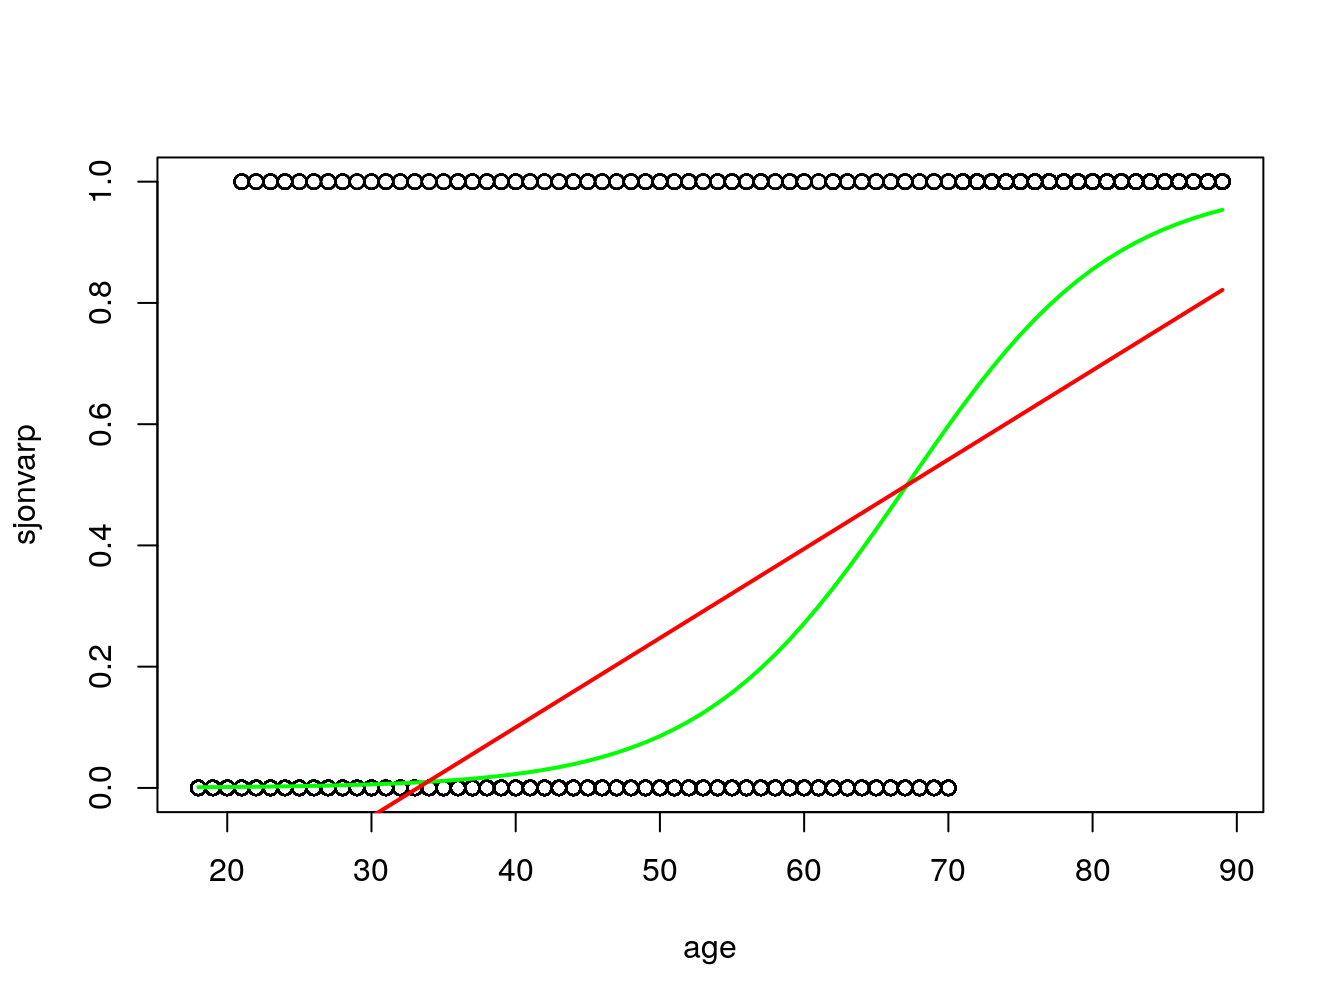
\includegraphics[width=0.8\linewidth]{timaglosur_files/figure-latex/two-models-1} 

}

\caption{Samanburður á línulegri aðfallsgreiningu og aðfallsgreiningu hlutfalla}\label{fig:two-models}
\end{figure}

Fyrir utan þennan alvarlega galla kemur það líka fyrir að leif líkans þar sem línuleg aðfallsgreining hefur verið notuð til að reikna samband milli einnar eða fleiri fumbreyta og einnar tvíkosta fylgibreytu, dreifst afbrigðilega með þeim afleiðingum að marktektarpróf sem byggja á líkaninu verða skekkt og gefa ranga mynd af aðstæðum í þýði.

\hypertarget{auxf0fallsgreining-hlutfalla-1}{%
\section{Aðfallsgreining hlutfalla}\label{auxf0fallsgreining-hlutfalla-1}}

Líkanið sem notað er fyrir aðfallsgreiningu hlutfalla lítur úr svona:

\(log(\frac{p}{1-p} ) \beta_{0}+\beta_{1}x\)

Þar sem \emph{p} er tvíliðu hlutfall (binomial proportion) og x er skýribreyta líkansins. Stikar líkansins fyrir eru \(\beta_{0}\) og \(\beta_{1}\).

Í línulegu líkani eru við að setja upp líkan þar sem meðaltal fylgibreytunnar veltur línulega á frumbreytu líkansins. Í aðfallsgreiningu hlutfalla er þetta meðaltal tekið af \emph{p} sem er þá fjöldi tilvika sem er með 1 á fylgibreytunni eða fjöldi successess. Í aðfallsgreiningu hlutfalla er markmiðið með líkaninu að finna meðaltal \emph{p} út frá frumbreytunni \emph{x}. Eins og við sáum áður þá er tæknilega hægt að gera þetta með línulegri aðfallsgreiningu en það veldur vandræðum þar sem í hvert skipti sem \(\beta_{0}\) tekur eitthvað annað gildi en 0 þá munu há gildi \emph{x} gefa spágildi (það er, \(\beta_{0}+\beta_{1}\)) sem falla utan mögulegra gilda \emph{p}, það er falla utan við spönnina frá 0 til 1. Það sem gert er með aðfallsgreiningu hlutfalla er að umbreyta hlutfallslíkunum með náttúrlegum lógarithma.

Þarna er gott að muna hvað hlutfallslíkur eru. Það má sjá hér: \ref{hl-likur}.

En það sem líkanið gerir er að það tekur fylgibreytuna (sem við táknum með \emph{y}, rétt eins og í línulegri aðfallsgreiningu) og umreiknar hana með náttúrlegum lógarithma og reiknar svo aðfallsgreiningu með þeim frumbreytum sem höfðu verið skilgreindar, það er, \emph{x} breyturnar. Á mynd \ref{fig:varlogreg} má sjá mismunandi líkön aðfallsgreiningar hlutfalla þar sem hallatölu líkansins er haldið stöðugri en skurðpunkti þess er breytt þannig að hann nái frá -16 upp í -4. Hins vegar má sjá á mynd \ref{fig:varlogreg2} hvernig tengsl breytanna líta út myndrænt þegar skurðpunktinum er haldið stöðugum en hallastuðlinum er breytt frá einu líkani til annars.

\begin{figure}

{\centering 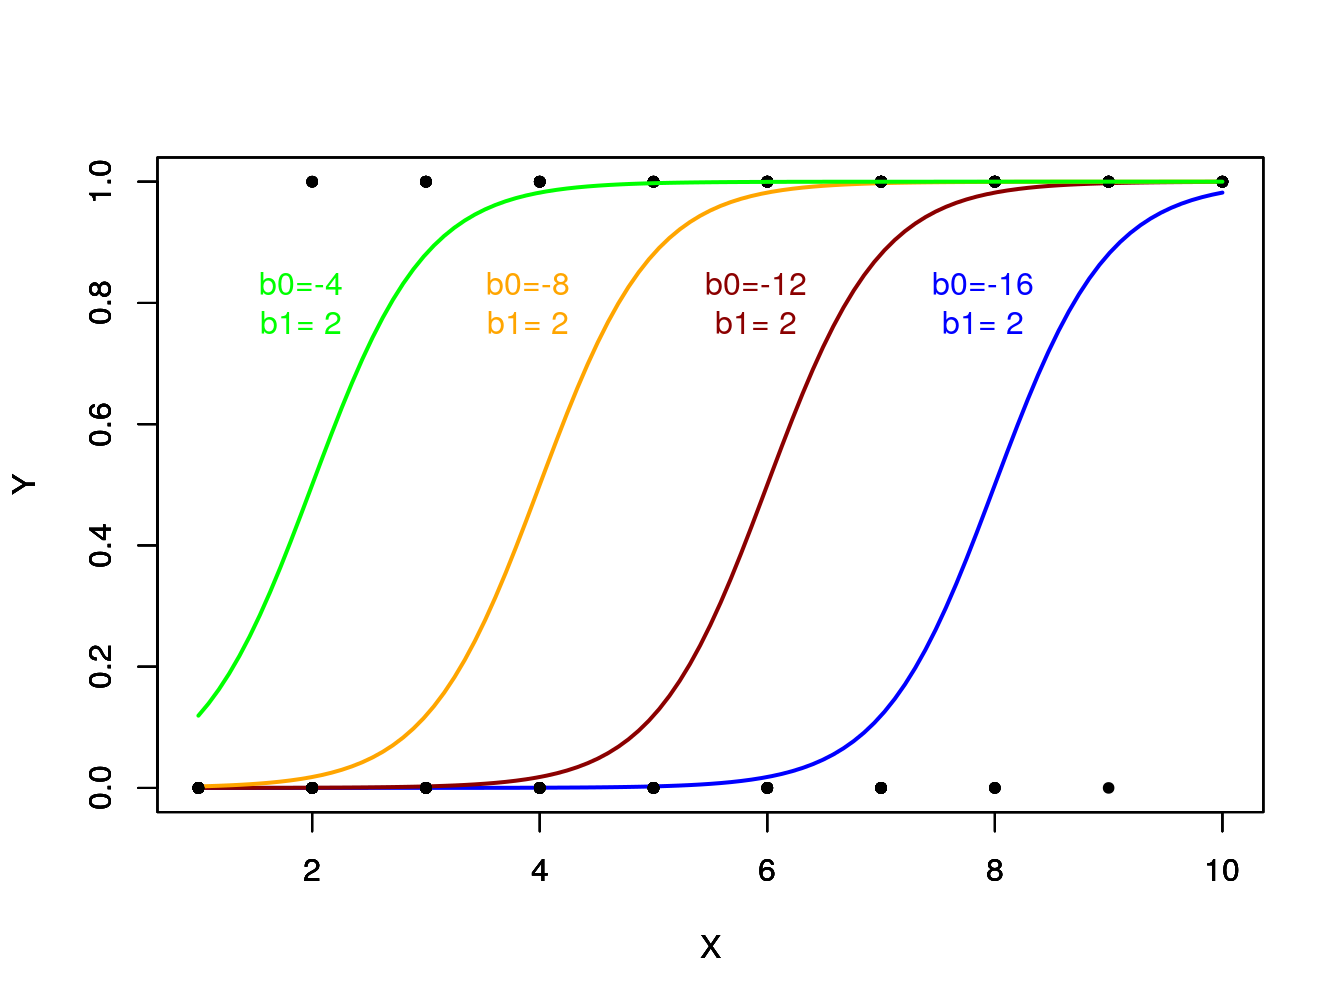
\includegraphics[width=0.8\linewidth]{timaglosur_files/figure-latex/varlogreg-1} 

}

\caption{Mismunandi líkön aðfallsgreiningar hlutfalla}\label{fig:varlogreg}
\end{figure}

\begin{figure}

{\centering 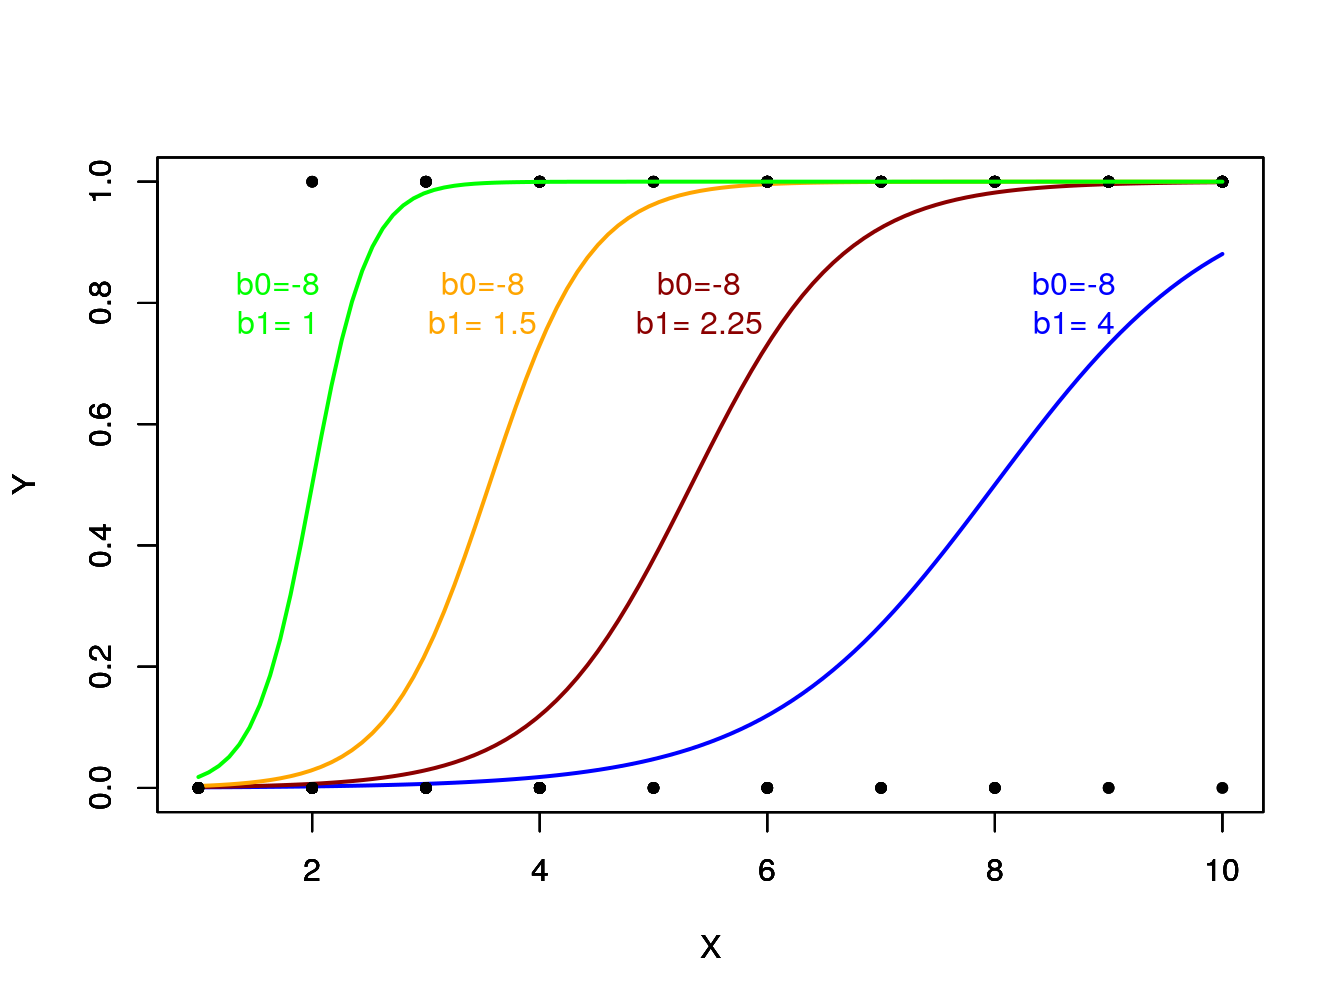
\includegraphics[width=0.8\linewidth]{timaglosur_files/figure-latex/varlogreg2-1} 

}

\caption{Mismunandi líkön aðfallsgreiningar hlutfalla}\label{fig:varlogreg2}
\end{figure}

\hypertarget{hvauxf0-er-nuxe1ttuxfarulegur-luxf3garithmi}{%
\subsection{Hvað er náttúrulegur lógarithmi?}\label{hvauxf0-er-nuxe1ttuxfarulegur-luxf3garithmi}}

Þegar við tökum náttúrlegan lógarithma af ákveðinni tölu þá er það gert með því að finna í hvaða veldi þarf að setja fastann \emph{e} til að útkoman verði upprunalega talan. Fastinn \emph{e} er einnig kallaður tala Eulers og er hún (í styttu formi) 2.7182818 Til dæmis má sjá að náttúrulegur lógarithmi af tölunni 3 er 1.0986123. Það merkir að til þess við verðum að setja fastann \emph{e} í 1.0986123 veldi til þess að hann verði 3, þar er: 3 \(= e^{log(3)}\)

Eins og áður segir er þetta skilgreiningin á náttúrulegum lógarithma en það er í raun hægt að taka lógarithma með því að nota hvaða jákvæða tölugildi sem er fyrir grunn lógarithmans. Til dæmis er algengt að taka lógarithma út frá grunninum 10. Góður kostur náttúrlegs lógarithma er að ef hann er tekinn af frum- eða fylgibreytu í aðfallsgreiningarlíkani þá er hægt að túlka umbreyttu breytuna á grunni prósentubreytinga. Til dæmis er fylgibreytu hefði verið umbreytt með náttúrulegum lógarithm í línulegri aðfallsgreiningu þá mætti túlka hallastuðul frumbreytu líkansins sem prósentubreytingu fylgibreytunnar.

Umbreytingu með lógarithma er stundum beitt til að temja ódæl gögn, til dæmis þegar forsenda aðfallsgreiningar um línulegt samband frum- og fylgibreyta virðist ekki standast. Við slíkar aðstæður gagnast oft prýðilega vel að umbreyta annað hvort frumbreytu eða fylgibreytu með lógarithma og veltur þá valið oft á því hvort breytan er skekktari.

Ein leið til að hugsa lógarithma er að hann dregur saman gögnin þannig að fjarlægðin milli gildanna á breytunni verður ekki eins mikil. Dæmi um þetta má sjá í töflu \ref{tab:logtafla}. Í töflunni má sjá að spönn hrágildanna er gríðarleg (frá 2 og uppí 50000) en þegar búið er að taka lógarithma þá eru tölurnar mun meðfærilegri og samþjappaðri þar sem spönnin er frá 0,69 og upp í 10,8. Þetta sama getum við séð þegar við tökum lógarithma af af hlutfallslíkum í aðfallsgreiningu hlutfalla - skalinn þjappast saman en samt þannig að fjarlægðin milli gildanna helst, hún minnkar bara.

\begin{table}

\caption{\label{tab:logtafla}Samanburður milli hrágagna og þar sem búið er að taka náttúrlegan lógarithma}
\centering
\begin{tabular}[t]{lrrrrrr}
\toprule
  & Fyrsta mæling & Önnur mæling & Þriðja mæling & Fjórða mæling & Fimmta mæling & Sjötta mæling\\
\midrule
hrágögn & 2.0000000 & 3.000000 & 7.00000 & 90.00000 & 1000.000000 & 50000.00000\\
logarithmi & 0.6931472 & 1.098612 & 1.94591 & 4.49981 & 6.907755 & 10.81978\\
\bottomrule
\end{tabular}
\end{table}

Samkvæmt hefðbundinni skilgreiningu er aðeins hægt að taka lógarithma af tölum sem eru hærri en 0 - þannig að undir venjulegum kringumstæðum er ekki hægt að taka lógarithma af núlli eða neikvæðum tölum.

Ef veldisvísisfall (exponential function) er tekið af tölu sem hefur verið umbreytt með lógarithma fæst upprunalega talan aftur. Þannig að \(exp(log(3))=3\).

\hypertarget{uppsetning-luxedkansins}{%
\subsection{Uppsetning líkansins}\label{uppsetning-luxedkansins}}

Líkanið sem við vinnum með í aðfallsgreiningu hlutfalla er eins og það sem við notum í línulegri aðfallsgreiningu. Eini munurinn er að spágildin eru ekki lengur meðaltal fyrir mismunandi gildi á frumbreytunni \emph{x} heldur lógarithmi hlutfallslíkinda fyrir mismunandi gildi frumbreytunnar \emph{x} í líkaninu.

\hypertarget{uxe1huxe6ttuhlutfall}{%
\subsection{Áhættuhlutfall}\label{uxe1huxe6ttuhlutfall}}

Þegar við fáum niðurstöður úr aðfallsgreiningu hlutfalla þá eru hallastuðlar allir á skala sem byggir á lógarithma hlutfallslíkinda. Það er hins vegar ekki þægilegt að túlka hallastuðla sem eru á þessum skala. Af þeirri ástæðu eru niðurstöðurnar yfirleitt alltaf unnar frekar og áhættuhlutfall reiknað.

Það sem heitir á ensku odds ratio er nefnt áhættuhlutfall á íslensku. Áhættuhlutfall er einfalt að túlka en það er nokkuð frábrugðið frá þeim hallastuðlum sem við erum vön úr línulegri aðfallsgreiningu.

Áhættuhlutfall er reiknað með því að taka anti-log eða veldisvísisfall af hallastuðlum líkansins. Með þessari aðgerð eru áhrif lógarithmans fjarlægð úr hallastuðlunum. Áhættuhlutfall er í raun hlutfallið milli tveggja hlutfallslíka. Spönn þess er frá 0 til óendanlegs. Ef áhættuhlutfallið er 1 þá er það til marks um að engin tengsl er milli breytanna. Ef það er hærra en 1 þá er sambandið jákvætt en ef það er lægra en 1 þá er sambandið neikvætt.

\hypertarget{tegundir-frumbreyta-uxed-auxf0fallsgreiningu-hlutfalla}{%
\subsection{Tegundir frumbreyta í aðfallsgreiningu hlutfalla}\label{tegundir-frumbreyta-uxed-auxf0fallsgreiningu-hlutfalla}}

Aðfallsgreining hlutfalla ræður bæði við samfelldar og flokkaðar frumbreytur. Sömu reglur gilda um notkun frumbreyta eins og fyrir línulega aðfallsgreiningu: Hægt er að nota samfelldar breytur beint af kúnni í líkanið en fyrir flokkabreytur þarf að ákvarða einn samanburðarhóp sem aðrir flokkar verða bornir saman við.

Þegar niðurstöðurnar eru túlkaðar út frá flokkuðum frumbreytum er það gert á grundvelli þess að miðað við viðmiðunarhópinn þá var sá hópur sem kemur fram í niðurstöðutöflunni með þeim mun hærra áhættuhlutfall að jafnaði eða lægra ef áhættuhlutfallið var lægra en 1.

Ef við værum til dæmis að bera saman kynin þar sem karlar væru kóðaðir sem 1 og konur sem 0 eftir líkindum þess að fá greiddar örorkubætur frá Tryggingastofnun, þá myndi áhættuhlutfallið 0,8 benda til þess að karla væru að jafnaði um 20\% ólíklegri en konur til að fá örorkubætur greiddar.

Að sama skapi ef við værum aftur að skoða kynin með sömu kóðun og áður nema út frá líkindum þess að hafa verið sviptur ökuréttindum einhverntíman á ævinni, þá myndi áhættuhlutfallið 1,35 benda til þess að karlar væru að jafnaði um 35\% líklegri en konur til að hafa tapað bílprófinu.

\hypertarget{duxf6nsk-uxedbuxfaakuxf6nnun}{%
\subsection{Dönsk íbúakönnun}\label{duxf6nsk-uxedbuxfaakuxf6nnun}}

Við erum með gagnasafn frá Kaupmannahöfn þar sem íbúar í borginni voru spurðir um tegundir húsnæðis, samskipti við nágranna sína og ánægju með húsnæði sitt. Það sem við höfum áhuga á að skoða eru tengslin milli þess hversu mikil samskipti svarendur höfðu við nágranna sína og hversu ánægðir þeir voru með húsnæði sitt. Gagnasafnið er fengið héðan: \url{https://data.princeton.edu/wws509/datasets/\#copen}

Breytan contact var til marks um hversu mikil samskipti svarendur höfðu við nágranna sína. Hún var kóðuð 1 þar sem samskipti voru mikil en 0 þar sem samskipti voru lítil.

Í upprunalega gagnasafninu var ánægja með húsnæðið mælt með þrískiptri breytu sem skiptis í lítið ánægðir, í meðallagi ánægðir og mjög ánægðir. Í greiningunni hér voru þeir teknir úr gagnasafninu sem voru í meðallagi ánægðir. Breytan var svo endurkóðuð þannig að þeir sem voru mjög ánægðir fengu gildið 1 en þeir sem voru lítið ánægðir fengu gildið 0.

Niðurstöður líkansins má sjá í töflu \ref{tab:kobentafla}. Þar má sjá tengsl frumbreytunnar við fylgibreytuna miðað við lógarithma hlutfallslíkinda, staðalvilluna, niðurstöður z-prófs og samsvarandi p-gildi.

\begin{table}

\caption{\label{tab:kobentafla}Niðurstöður aðfallsgreiningar hlutfalla}
\centering
\begin{tabular}[t]{l|r|r|r|r}
\hline
  & Stuðull & Staðalvilla & z-gildi & p-gildi\\
\hline
Skurðpunktur & 0.04 & 0.09 & 0.48 & 0.63\\
\hline
Samskipti við nágranna & 0.22 & 0.12 & 1.89 & 0.06\\
\hline
\end{tabular}
\end{table}

Í töflu \ref{tab:kobentafla2} má hins vegar sjá þegar búið er að hreinsa lógarithman úr niðurstöðunum og þá kemur í ljós áhættuhlutfallið auk öryggsibilsins fyrir áhættuhlutfallið. Samkvæmt þessum niðurstöðum eru þeir sem eiga mikil samskipti við nágranna sína um 22\% líklegri til að vera mjög ánægðir með húsnæðiskost sinn, miðað við þá sem áttu í litlum samskiptum við nágranna. Hins vegar er einnig rétt að skoða öryggisbilið sem bendir til að ekki sé víst að um sé að ræða mun sem á sér stoð í þýðinu þar sem öryggisbil áhættuhlutfallsins inniheldur 1 og eins og við munum þá stendur 1 fyrir engin tengsl milli frum -og fylgibreytu líkansins.

\begin{table}

\caption{\label{tab:kobentafla2}Niðurstöður aðfallsgreiningar hlutfalla}
\centering
\begin{tabular}[t]{l|r|r|r|l}
\hline
Frumbreyta & Áhættuhlutfall & Öryggisbil neðra & Öryggisbil efra & Kvarði breytunnar\\
\hline
Samskipti við nágranna & 1.24 & 0.99 & 1.56 & Indicator variable\\
\hline
\end{tabular}
\end{table}

Mikilvægt er að ef hópum frumbreytunnar hefði verið snúið við (það er, þeir sem voru í miklum samskiptum við nágranna hefðu fengið 0 og þeir sem voru í litlum samskiptum fengið 1) þá hefði áhættuhlutfallið breyst. Þær niðurstöður má sjá í töflu \ref{tab:kobentafla3}. Þá má sjá að ef við notum þá sem voru í miklum samskiptum við nágranna sína sem viðmiðunarhóp þá voru þeir sem voru í litlum samskiptum að jafnaði um 20\% ólíklegri til að vera ánægðir með húsnæðisstöðu sína, miðað við samanburðarhópinn.

\begin{table}

\caption{\label{tab:kobentafla3}Niðurstöður aðfallsgreiningar hlutfalla - breytt kóðun frumbreytunnar}
\centering
\begin{tabular}[t]{l|r|r|r|l}
\hline
Frumbreyta & Áhættuhlutfall & Öryggisbil neðra & Öryggisbil efra & Kvarði breytunnar\\
\hline
Samskipti við nágranna & 0.8 & 0.64 & 1.01 & Indicator variable\\
\hline
\end{tabular}
\end{table}

\hypertarget{uxe1lyktun-uxe1-grundvelli-auxf0fallsgreiningar-hlutfalla}{%
\section{Ályktun á grundvelli aðfallsgreiningar hlutfalla}\label{uxe1lyktun-uxe1-grundvelli-auxf0fallsgreiningar-hlutfalla}}

Nú er gott að rifja upp hvernig líkanið fyrir aðfallsgreiningu hlutfalla lítur út:

\(log(\frac{p}{1-p} ) \beta_{0}+\beta_{1}x\)

Þar sem \emph{p} er tvíliðu hlutfall (binomial proportion) og x er skýribreyta líkansins. Stikar líkansins fyrir eru \(\beta_{0}\) og \(\beta_{1}\).

Það kallar á talsverða vinnu (og helst sérhæfðan hugbúnað) að reikna aðfallsgreiningu hlutfalla í höndunum. Ein undantekning á þessu er ef um er að ræða líkan með einni tvískiptri frumbreytu. Í því tilfelli getum við auðveldlega reiknað hallastuðulinn og skurðpunktinn.

Ef við skoðum dæmið sem við tókum áður út frá dönsku íbúakönnuninni þá líta formúlunar svona út:

\begin{itemize}
\tightlist
\item
  Formúla fyrir aðfallsgreiningu hlutfalla fyrir þá sem höfðu mikil samskipti við nágranna sína
\end{itemize}

\(log(\frac{p_{samskipti} }{1-p_{samskipti}} )=\beta_{0}+\beta_{1}\)

\begin{itemize}
\tightlist
\item
  Formúla fyrir þá sem höfðu lítil samskipti við nágranna sína
\end{itemize}

\(log(\frac{p_{lítilsamskipti} }{1-p_{lítilsamskipti}} )=\beta_{0}\)

Út frá þessu sjáum við að matið fyrir skurðpunkt líkansins er það sama og matið á hlutfallslíkum þeirra sem eiga lítil samskipti við nágranna sína. Við sjáum líka að til að reikna mat á hallastuðli líkansins þá þarf að finna mismuninn milli hlutfallslíka hópanna tveggja. Við getum reiknað hlutfallslíkurnar og sjáum að þær eru 0.258574 fyrir þá sem eiga í mikum samskiptum við nágranna og 0.0411273 fyrir hina.

Út frá þessu getum við reiknað hallastuðul líkansins

\(\beta_{1}=\) 0.2174467

Eins og við vitum þá er hann illtúlkanlegur og því viljum við taka antilog af honum. Þá verður niðurstaðan 1.2428992.

Ályktunartölfræði er reiknuð með sama hætti fyrir aðfallsgreiningu hlutfalla rétt eins og fyrir línulega aðfallsgreiningu. Mat á stikum er reiknað fyrir líkanið og staðalvilla er metin fyrir þá.

\hypertarget{uxf6ryggisbil}{%
\subsection{Öryggisbil}\label{uxf6ryggisbil}}

Öryggisbil eru reiknuð á hefðbundinn hátt, nema miðað er við normaldreifingu í stað t-dreifingar, sem er sú dreifing sem miðað er við í línulegri aðfallsgreiningu.
Öryggisbil fyrir hallastuðla er: \(b_{1} \pm z^\ast SE_{b1}\)

Fyrir hlutfallslíkur er öryggisbilið reiknað með að umbreyta öryggisbilinu með því að taka antilog af því. Það er gert svohljóðandi: \((e^{b_{1}-z^\ast SE_{b_{1} } }, e^{b_{1}+z^\ast SE_{b_{1} } })\) þar sem \(z^*\) stendur fyrir normal þéttleikakúrvu með svæðið C (sem er öryggisbilið sem miðað er við) milli \(-z^*\) og \(+z^*\).

Þegar um er að ræða hlutfallslíkur þá skoðum við grant hvort öryggisbilið nái utan um 1, þar sem 1 er til marks um að enginn munur sé á hlutföllum hópanna sem við erum að skoða (þegar um er að ræða tvíkosta frumbreytu) eða að engin tengsl séu milli frumbreytunnar og fylgibreytunnar (þegar við erum með samfellda frumbreytu). Ef öryggisbilið inniheldur gildið 1 þá getum við ekki verið viss um að tengsl séu til staðar í þýðinu.

\hypertarget{marktektarpruxf3f}{%
\subsection{Marktektarpróf}\label{marktektarpruxf3f}}

Marktektarpróf eru unnin út frá hlutfallinu milli hallastuðulsins og staðalvillunnar. Oft eru niðurstöður marktektarprófanna gefnar sem veldistölur þessara niðurstaðna (það er, squared niðurstöður). Í þeim tilvikum er um að ræða p-gildi út frá kí-kvaðrat dreifingunni með n-1 frígráðu.

Til að prófa hvort hallatalan sé marktækt ólík 0 (það er, hvort líklegt sé að fá hallatölu af þessum styrkleika ef ekki er um að ræða tengsl í þýði) er eftirfarandi próf framvkæmt:

\(z=\frac{b_1}{SE_{b_{1}}}\)

Þetta gildi er borið saman við z-gildi út frá normaldreifingu. Það er nokkuð flókið að reikna út staðalvillu fyrir stika í aðfallsgreiningu hlutfalla og því látum við hugbúnaðinn um það verkefni.

Þetta próf er kallað Wald próf en í sumum tilvikum reiknar tölfræðihugbúnaður kíkvaðrat próf til að próf hvort um sé að ræða marktækan hallastuðul eða ekki. Það er veltur á því að: \(\chi^2=z^2\)

Þar sem við erum jafnan að vinna með hlutfallslíkur þá breytist marktektarprófið í að verða próf á því hvort hlutfallslíkindin víki marktækt frá 1. Það er, hlutfallslíkindi sem eru 1 er til marks um að enginn munur sé á hlutföllum tveggja hópanna (ef um er að ræða tvískipta frumbreytu). Þess vegna er núlltilgátan í þessu tilviki að hlutfallslíkindin eru 1. Aðaltilgátan er þá að hlutfallslíkindin séu einhver önnur en 1 - það er, að munur sé á hópunum.

\hypertarget{duxe6mi}{%
\subsection{Dæmi}\label{duxe6mi}}

Gögnin sem við notum til að skoða aðfallsgreiningu hlutfalla kemur úr manntali bandaríkjanna frá árinu 1994. Eftirfarandi breytur er að finna í gagnasafninu:

Frumbreytur:

\begin{itemize}
\tightlist
\item
  age: continuous.
\item
  workclass: Private, Self-emp-not-inc, Self-emp-inc, Federal-gov, Local-gov, State-gov, Without-pay, Never-worked.
\item
  fnlwgt: continuous.
\item
  education: Bachelors, Some-college, 11th, HS-grad, Prof-school, Assoc-acdm, - Assoc-voc, 9th, 7th-8th, 12th, Masters, 1st-4th, 10th, Doctorate, 5th-6th, Preschool.
\item
  education-num: continuous.
\item
  marital-status: Married-civ-spouse, Divorced, Never-married, Separated, Widowed, Married-spouse-absent, Married-AF-spouse.
\item
  occupation: Tech-support, Craft-repair, Other-service, Sales, Exec-managerial, Prof-specialty, Handlers-cleaners, Machine-op-inspct, Adm-clerical, Farming-fishing, Transport-moving, Priv-house-serv, Protective-serv, Armed-Forces.
\item
  relationship: Wife, Own-child, Husband, Not-in-family, Other-relative, Unmarried.
\item
  race: White, Asian-Pac-Islander, Amer-Indian-Eskimo, Other, Black.
\item
  sex: Female, Male.
\item
  capital-gain: continuous.
\item
  capital-loss: continuous.
\item
  hours-per-week: continuous.
\item
  native-country: United-States, Cambodia, England, Puerto-Rico, Canada, Germany, Outlying-US(Guam-USVI-etc), India, Japan, Greece, South, China, Cuba, Iran, Honduras, Philippines, Italy, Poland, Jamaica, Vietnam, Mexico, Portugal, Ireland, France, Dominican-Republic, Laos, Ecuador, Taiwan, Haiti, Columbia, Hungary, Guatemala, Nicaragua, Scotland, Thailand, Yugoslavia, El-Salvador, Trinadad\&Tobago, Peru, Hong, Holand-Netherlands.
\end{itemize}

Fylgibreytan:
- income: \textgreater{}50K, \textless{}=50K

Frekari upplýsingar og gagnasafnið sjálft má nálgast hér: \url{https://archive.ics.uci.edu/ml/datasets/census+income}

Okkar verkefni er að skoða hvort munur sé á líkum þess að tekjur fólks séu hærri eða lægri en 50 þúsund dalir á ári eftir því hvort um er að ræða karl eða konu. Fyrsta verkefni okkar er að endurreikna báðar breytur þannig að þær séu báðar tvíkosta og innihaldi aðeins gildin 0 og 1.

\begin{Shaded}
\begin{Highlighting}[]
\KeywordTok{library}\NormalTok{(tidyverse)}

\CommentTok{#Fyrst lesa gögnin inn í R}
\NormalTok{gogn =}\StringTok{ }\KeywordTok{read.delim}\NormalTok{(}\DataTypeTok{file=}\StringTok{"~/kennsla/2019/Tölfræði III/tolfr3/timaglosur/adult.data"}
\NormalTok{                  , }\DataTypeTok{sep =} \StringTok{","}\NormalTok{, }\DataTypeTok{header =} \OtherTok{FALSE}\NormalTok{)}

\CommentTok{#setja nöfn á allar breyturnar í settinu. }
\CommentTok{#Þegar unnið er með gagnaskrá af gerðinni dat þarf jafnan að gera það.}
\KeywordTok{names}\NormalTok{(gogn) =}\StringTok{ }\KeywordTok{c}\NormalTok{(}\StringTok{"age"}\NormalTok{,}\StringTok{"workclass"}\NormalTok{,}\StringTok{"fnlwgt"}\NormalTok{,}\StringTok{"education"}\NormalTok{,}\StringTok{"education_num"}
\NormalTok{                ,}\StringTok{"marital_status"}\NormalTok{,}\StringTok{"occupation"}\NormalTok{,}\StringTok{"relationship"}\NormalTok{,}\StringTok{"race"}
\NormalTok{                ,}\StringTok{"sex"}\NormalTok{,}\StringTok{"capital_gain"}\NormalTok{,}\StringTok{"capital_loss"}\NormalTok{,}\StringTok{"hours_per_week"}
\NormalTok{                ,}\StringTok{"native_country"}\NormalTok{,}\StringTok{"income"}\NormalTok{)}

\CommentTok{#loks eru frumbreytan og fylgibreytan endurkóðaðar til að taka aðeins gildin 0 og 1.}

\CommentTok{#fyrst skoðum við núverandi gildi breytunnar}
\KeywordTok{table}\NormalTok{(gogn}\OperatorTok{$}\NormalTok{income)}
\end{Highlighting}
\end{Shaded}

\begin{verbatim}
## 
##  <=50K   >50K 
##  24720   7841
\end{verbatim}

\begin{Shaded}
\begin{Highlighting}[]
\NormalTok{gogn}\OperatorTok{$}\NormalTok{income =}\StringTok{ }\KeywordTok{as.numeric}\NormalTok{(gogn}\OperatorTok{$}\NormalTok{income)}\OperatorTok{-}\DecValTok{1}
\CommentTok{#og svo skoðum við gildi breytunnar eftir umbreytingu}
\KeywordTok{table}\NormalTok{(gogn}\OperatorTok{$}\NormalTok{income)}
\end{Highlighting}
\end{Shaded}

\begin{verbatim}
## 
##     0     1 
## 24720  7841
\end{verbatim}

\begin{Shaded}
\begin{Highlighting}[]
\CommentTok{#hér viljum við að 0 sé fyrir þá sem eru með árstekjur }
\CommentTok{#undir 50 þúsund dölum en þeir sem eru með hærri tekjur }
\CommentTok{#eiga að fá gildið 1.}


\CommentTok{#svo endurkóðum við kynjabreytuna þannig að konur fái gildið 1 en karlar fái gildið 0}
\NormalTok{gogn }\OperatorTok\StringTok{ }
\StringTok{  }\KeywordTok{count}\NormalTok{(sex)}
\end{Highlighting}
\end{Shaded}

\begin{verbatim}
## # A tibble: 2 x 2
##   sex           n
##   <fct>     <int>
## 1 " Female" 10771
## 2 " Male"   21790
\end{verbatim}

\begin{Shaded}
\begin{Highlighting}[]
\CommentTok{#hérna endurkóðum við kynjabreytuna með tidyverse}
\NormalTok{gogn =}\StringTok{ }\NormalTok{gogn }\OperatorTok
\StringTok{  }\KeywordTok{mutate}\NormalTok{(}\DataTypeTok{sex=}\KeywordTok{ifelse}\NormalTok{(sex }\OperatorTok{==}\StringTok{ ' Female'}\NormalTok{, }\DecValTok{1}\NormalTok{, }\DecValTok{0}\NormalTok{))}

\NormalTok{gogn}\OperatorTok{$}\NormalTok{sex =}\StringTok{ }\KeywordTok{as.factor}\NormalTok{(gogn}\OperatorTok{$}\NormalTok{sex)}
\end{Highlighting}
\end{Shaded}

Þegar því er lokið má hefja greininguna.

\begin{Shaded}
\begin{Highlighting}[]
\CommentTok{#hér er líkanið skilgreint}
\CommentTok{#default stillingin er línileg aðfallsgreining og þess vegna þarf að breyta family í binomial}

\NormalTok{likan1 =}\StringTok{ }\KeywordTok{glm}\NormalTok{(income}\OperatorTok{~}\NormalTok{sex, }\DataTypeTok{family=}\StringTok{"binomial"}\NormalTok{, }\DataTypeTok{data=}\NormalTok{gogn)}

\CommentTok{#hér sjáum við svo hráar niðurstöður líkansins. }
\CommentTok{#Takið eftir að hér er ekki búið að umreikna hallastuðulinn }
\CommentTok{#þannig að hann er enn á lógarithma skala.}
\KeywordTok{summary}\NormalTok{(likan1)}
\end{Highlighting}
\end{Shaded}

\begin{verbatim}
## 
## Call:
## glm(formula = income ~ sex, family = "binomial", data = gogn)
## 
## Deviance Residuals: 
##     Min       1Q   Median       3Q      Max  
## -0.8543  -0.8543  -0.4815  -0.4815   2.1034  
## 
## Coefficients:
##             Estimate Std. Error z value Pr(>|z|)    
## (Intercept) -0.82013    0.01470  -55.78   <2e-16 ***
## sex1        -1.27614    0.03418  -37.33   <2e-16 ***
## ---
## Signif. codes:  0 '***' 0.001 '**' 0.01 '*' 0.05 '.' 0.1 ' ' 1
## 
## (Dispersion parameter for binomial family taken to be 1)
## 
##     Null deviance: 35948  on 32560  degrees of freedom
## Residual deviance: 34270  on 32559  degrees of freedom
## AIC: 34274
## 
## Number of Fisher Scoring iterations: 4
\end{verbatim}

\begin{table}

\caption{\label{tab:tekjutafla1}Samband kyns og tekna samkvæmt manntalinu 1996}
\centering
\begin{tabular}[t]{l|r|r|r|l}
\hline
Frumbreyta & Áhættuhlutfall & Öryggisbil neðra & Öryggisbil efra & Kvarði breytunnar\\
\hline
Kyn & 0.28 & 0.26 & 0.3 & Indicator variable\\
\hline
\end{tabular}
\end{table}

Í töflu \ref{tab:tekjutafla1} sjáum við niðurstöður líkansins þar sem spáð tengslin milli kyns og tekna eru skoðuð og þar sem búið er að umbreyta hallastuðli líkansins í áhættuhlutfall. Við vildum við vita hvort líkurnar á að vera með hærri árstekjur en 50 þúsund dollarar tengdust kyni. Hér sjáum við að konur er að jafnaði um 72\% ólíklegri en karlar til að vera með árstekjur hærri en 50 þúsund dollarar, og 95\% öryggisbilið nær frá 70 - 74\%. Þetta er semsg

Þetta er semsagt nokkuð nákvæmt mat, sem skýrist meðal annars af því hversu stórt úrtakið er (n = 32561). Ennfremur inniheldur öryggisbilið ekki 1 sem bendir til þess að líklega eru tengslin til staðar í þýðinu. Það má einnig sjá af hráau niðurstöðum líkansins úr R en þar mátti sjá marktækt Wald próf fyrir hallastuðulinn.

\hypertarget{sennileikahlutfall}{%
\section{Sennileikahlutfall}\label{sennileikahlutfall}}

Wald prófið er notað til að kanna, fyri hvern og einn stika, hvort þeir séu marktækir eða ekki út frá \(\chi^2\)-dreifingu með einni frígráðu. Þetta er einfalt próf en kann að vera bjagað, sérstaklega þegar um er að ræða lítil úrtök. Þegar um er að ræða niðurstöður með háu stikamati er staðalvillan oft ofmetin og þá verður gildi Wald prófsins vanmetið. Í þeim tilvikum getur Wald prófið bent til þess frumbreytan sem um ræðir skipti litlu eða engu máli fyrir forspá fylgibreytunnar.

Af þessari ástæðu getur verið betra að nota sennileikahlutfall (likelihood ratio). Mælst er gegn því að nota gervi-\(R^2\) þar sem þeir gefa yfirleitt ekki raunsanna mynd af gæðum líkansins.

Hér sjáum við formúlu sennileikahlutfallsprófsins:

\(-2 \times ln(lr) = -2\times ln({L_{0}}/{L_{1}} )\)
eða
\(-2 \times ln(lr) = -2\times (lnL_{0}-lnL_{1} )\)

Það sem þetta þýðir er að tvö líkön eru borin saman, annars vegar líkan sem er aðeins með skurðpunkti (sem er táknað sem \(L_0\)) og svo líkan þar sem hallastuðli hefur verið bætt við (sem er táknað sem \(L_1\)). Með þessu getum við metið að hvaða marki mátgæði líkansins við gögnin batna við að setja hverja frumbreytu í líkanið.

Gott er að bera saman niðurstöður Wald prófs fyrir hverja frumbreytu fyrir sig og niðurstöður sennileikahlutfallsins. Við getum skoðað dæmi þar sem við skáldum upp gögn sem líklegt er að hafi áhrif á niðurstöður Wald prófsins.

\begin{figure}
\centering
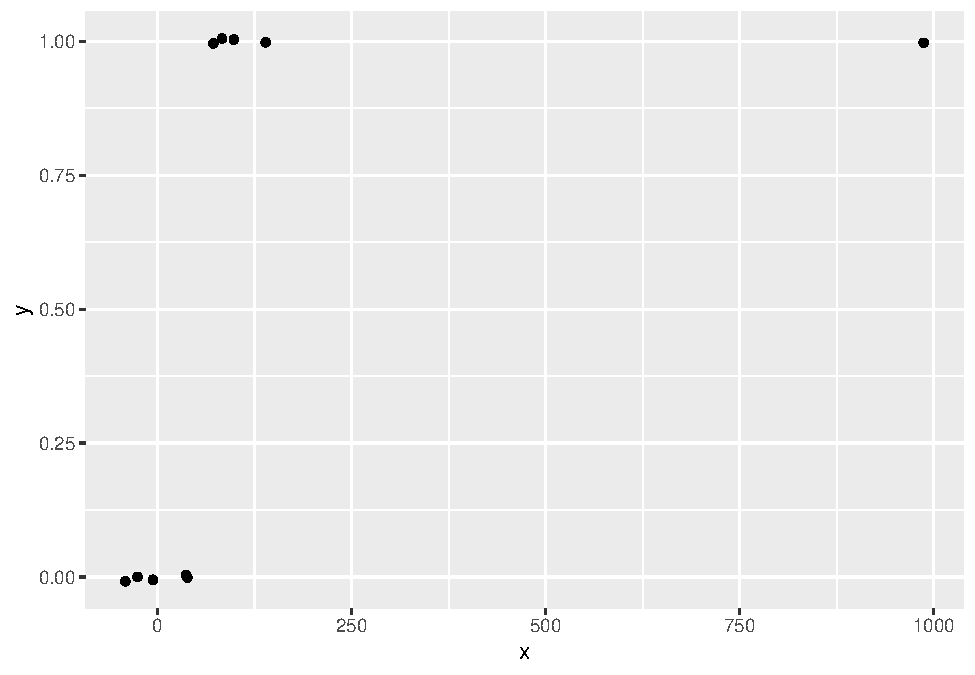
\includegraphics{timaglosur_files/figure-latex/lrtestmynd-1.pdf}
\caption{\label{fig:lrtestmynd}Sambandið milli x og y}
\end{figure}

Á mynd \ref{fig:lrtestmynd} sjáum við samband tveggja breyta, x og y. Við reiknum aðfallsgreiningu hlutfalla, niðurstöðurnar má sjá í töflu \ref{tab:taflaxy}. Eins og sjá má er Wald-prófið langt, langt frá því að vera marktækt og p-gildið er nánast 1.

\begin{table}

\caption{\label{tab:taflaxy}Aðfallsgreining hlutfalla milli x og y}
\centering
\begin{tabular}[t]{l|r|r|r|r}
\hline
  & Stuðlar & Staðalvilla & Wald próf & p-gildi\\
\hline
(Intercept) & -27.10781 & 37673.330 & -0.00072 & 0.99943\\
\hline
x & 0.99102 & 1028.555 & 0.00096 & 0.99923\\
\hline
\end{tabular}
\end{table}

Ef við reiknum hins vegar sennileikahlutfallspróf þá fáum við allt aðra niðurstöðu; marktækt kí-kvaðrat próf.

\begin{Shaded}
\begin{Highlighting}[]
\KeywordTok{lrtest}\NormalTok{(likan2)}
\end{Highlighting}
\end{Shaded}

\begin{verbatim}
## Likelihood ratio test
## 
## Model 1: y ~ x
## Model 2: y ~ 1
##   #Df  LogLik Df  Chisq Pr(>Chisq)    
## 1   2  0.0000                         
## 2   1 -6.9315 -1 13.863  0.0001966 ***
## ---
## Signif. codes:  0 '***' 0.001 '**' 0.01 '*' 0.05 '.' 0.1 ' ' 1
\end{verbatim}

Að auki má geta þess að mælt er með því að nota Hosmer-Lemeshow prófið til að kanna mátgæði líkana sem byggja á aðfallsgreiningu hlutfalla. Í prófinu eru raunmælingar fylgibreytunnar bornar saman við væntigildi líkansins. Prófið gefur til kynna ef munurinn milli mældra gilda og væntigilda út frá líkaninu sé marktækuyr eða ekki. Ef þessi munur er markæktur þá er það til marks um að mátgæði líkansins sé ábótavant. Það eru hins vegar ákveðnir ágallar á Hosmer-Lemeshow prófinu og því eru til enn nýrri aðferðir til að skoða mátgæði mismunandi líkana, til dæmis \emph{le Cessie--van Houwelingen--Copas--Hosmer unweighted sum of squares test}.

\hypertarget{fjuxf6lbreytu-auxf0fallsgreining-hlutfalla}{%
\section{Fjölbreytu aðfallsgreining hlutfalla}\label{fjuxf6lbreytu-auxf0fallsgreining-hlutfalla}}

Fjölbreytu aðfallsgreining hlutfalla er afar svipuð og þegar marghliða aðfallgreining er framkvæmd. Við bætum við fleiri frumbreytum og reynum með því að stjórna tölfræðilega fyrir áhrifum þeirra á fylgibreytuna. Það verður því alltaf að hafa í huga þegar við túlkum niðurstöðurnar.

VIð ætlum að nota sama gagnasafn og áður, það sem snýr að bandaríska manntalinu árið 1996. Við ætlum að bæta einni skýringarbreytu við líkanið og athuga hvort það hafi einhver áhrif á kynjamuninn sem við sáum fyrr. Í þessu tilviki ætlum við að bæta aldri við líkanið.

\begin{Shaded}
\begin{Highlighting}[]
\CommentTok{#hér er líkanið skilgreint}
\CommentTok{#default stillingin er línileg aðfallsgreining og þess vegna þarf að breyta family í binomial}

\NormalTok{likan1 =}\StringTok{ }\KeywordTok{glm}\NormalTok{(income}\OperatorTok{~}\NormalTok{sex}\OperatorTok{+}\NormalTok{age, }\DataTypeTok{family=}\StringTok{"binomial"}\NormalTok{, }\DataTypeTok{data=}\NormalTok{gogn)}

\CommentTok{#hér sjáum við svo hráar niðurstöður líkansins. }
\CommentTok{#Takið eftir að hér er ekki búið að umreikna hallastuðulinn }
\CommentTok{#þannig að hann er enn á lógarithma skala.}
\KeywordTok{summary}\NormalTok{(likan1)}
\end{Highlighting}
\end{Shaded}

\begin{verbatim}
## 
## Call:
## glm(formula = income ~ sex + age, family = "binomial", data = gogn)
## 
## Deviance Residuals: 
##     Min       1Q   Median       3Q      Max  
## -1.6685  -0.7648  -0.5887  -0.3190   2.4357  
## 
## Coefficients:
##              Estimate Std. Error z value Pr(>|z|)    
## (Intercept) -2.406572   0.044440  -54.15   <2e-16 ***
## sex1        -1.248412   0.034925  -35.75   <2e-16 ***
## age          0.039029   0.001002   38.94   <2e-16 ***
## ---
## Signif. codes:  0 '***' 0.001 '**' 0.01 '*' 0.05 '.' 0.1 ' ' 1
## 
## (Dispersion parameter for binomial family taken to be 1)
## 
##     Null deviance: 35948  on 32560  degrees of freedom
## Residual deviance: 32688  on 32558  degrees of freedom
## AIC: 32694
## 
## Number of Fisher Scoring iterations: 4
\end{verbatim}

\begin{table}

\caption{\label{tab:tekjutafla2}Samband kyns og aldurs við tekjur samkvæmt manntalinu 1996}
\centering
\begin{tabular}[t]{l|r|r|r|l}
\hline
Frumbreyta & Áhættuhlutfall & Öryggisbil neðra & Öryggisbil efra & Kvarði breytunnar\\
\hline
Kyn & 0.287 & 0.268 & 0.307 & Indicator variable\\
\hline
Aldur & 1.040 & 1.038 & 1.042 & 1\\
\hline
\end{tabular}
\end{table}

Við sjáum í töflu \ref{tab:tekjutafla2} að kyn hefur enn marktæk tengsl við tekjur en það lækkar lítillega miðað við það sem við sáum áður. Aldur hefur hins vegar einnig tengsl við árstekjur á þann hátt að fyrir hvert aldursár, þá aukast líkurnar á því að vera með hærri en 50 þúsund dali í árstekjur að jafnaði um 4\%, að teknu tilliti til áhrifa kyns. Öryggisbilið fyrir áhrif aldurs eru á bilinu 3,8 - 4,2\%.

Til gamans getum við bætt við annarri samfelldri frumbreytu í líkanið: Fjöldi ára í námi.

\begin{Shaded}
\begin{Highlighting}[]
\CommentTok{#hér er líkanið skilgreint}
\CommentTok{#default stillingin er línileg aðfallsgreining og þess vegna þarf að breyta family í binomial}

\NormalTok{likan1 =}\StringTok{ }\KeywordTok{glm}\NormalTok{(income}\OperatorTok{~}\NormalTok{sex}\OperatorTok{+}\NormalTok{age}\OperatorTok{+}\NormalTok{education_num, }\DataTypeTok{family=}\StringTok{"binomial"}\NormalTok{, }\DataTypeTok{data=}\NormalTok{gogn)}

\CommentTok{#hér sjáum við svo hráar niðurstöður líkansins. }
\CommentTok{#Takið eftir að hér er ekki búið að umreikna hallastuðulinn }
\CommentTok{#þannig að hann er enn á lógarithma skala.}
\KeywordTok{summary}\NormalTok{(likan1)}
\end{Highlighting}
\end{Shaded}

\begin{verbatim}
## 
## Call:
## glm(formula = income ~ sex + age + education_num, family = "binomial", 
##     data = gogn)
## 
## Deviance Residuals: 
##     Min       1Q   Median       3Q      Max  
## -2.4206  -0.6719  -0.4438  -0.1404   3.2565  
## 
## Coefficients:
##                Estimate Std. Error z value Pr(>|z|)    
## (Intercept)   -6.445691   0.090355  -71.34   <2e-16 ***
## sex1          -1.323611   0.036840  -35.93   <2e-16 ***
## age            0.042613   0.001133   37.62   <2e-16 ***
## education_num  0.369457   0.006539   56.50   <2e-16 ***
## ---
## Signif. codes:  0 '***' 0.001 '**' 0.01 '*' 0.05 '.' 0.1 ' ' 1
## 
## (Dispersion parameter for binomial family taken to be 1)
## 
##     Null deviance: 35948  on 32560  degrees of freedom
## Residual deviance: 28718  on 32557  degrees of freedom
## AIC: 28726
## 
## Number of Fisher Scoring iterations: 5
\end{verbatim}

\begin{table}

\caption{\label{tab:tekjutafla3}Samband kyns, aldurs og menntunar við tekjur samkvæmt manntalinu 1996}
\centering
\begin{tabular}[t]{l|r|r|r|l}
\hline
Frumbreyta & Áhættuhlutfall & Öryggisbil neðra & Öryggisbil efra & Kvarði breytunnar\\
\hline
Kyn & 0.266 & 0.248 & 0.286 & Indicator variable\\
\hline
Aldur & 1.044 & 1.041 & 1.046 & 1\\
\hline
FJöldi ára í námi & 1.447 & 1.429 & 1.466 & 1\\
\hline
\end{tabular}
\end{table}

Að lokum skoðum við hvernig tengslin milli tekna og menntunar líta út myndrænt.

\begin{Shaded}
\begin{Highlighting}[]
\NormalTok{fit =}\StringTok{ }\KeywordTok{glm}\NormalTok{(income }\OperatorTok{~}\StringTok{ }\NormalTok{education_num, }\DataTypeTok{data=}\NormalTok{gogn, }\DataTypeTok{family=}\NormalTok{binomial)}
\NormalTok{newdat <-}\StringTok{ }\KeywordTok{data.frame}\NormalTok{(}\DataTypeTok{education_num=}\KeywordTok{seq}\NormalTok{(}\KeywordTok{min}\NormalTok{(gogn}\OperatorTok{$}\NormalTok{education_num), }\KeywordTok{max}\NormalTok{(gogn}\OperatorTok{$}\NormalTok{education_num),}\DataTypeTok{len=}\DecValTok{100}\NormalTok{))}

\NormalTok{newdat}\OperatorTok{$}\NormalTok{income =}\StringTok{ }\KeywordTok{predict}\NormalTok{(fit, }\DataTypeTok{newdata=}\NormalTok{newdat, }\DataTypeTok{type=}\StringTok{"response"}\NormalTok{)}

\KeywordTok{plot}\NormalTok{(}\KeywordTok{jitter}\NormalTok{(income,}\DecValTok{1}\NormalTok{)}\OperatorTok{~}\KeywordTok{jitter}\NormalTok{(education_num, }\DecValTok{1}\NormalTok{), }\DataTypeTok{data=}\NormalTok{gogn, }\DataTypeTok{col=}\StringTok{"red4"}\NormalTok{, }\DataTypeTok{ylab =} \StringTok{"Tekjur"}\NormalTok{, }\DataTypeTok{xlab =} \StringTok{"Menntun"}\NormalTok{)}
\KeywordTok{lines}\NormalTok{(income }\OperatorTok{~}\StringTok{ }\NormalTok{education_num, newdat, }\DataTypeTok{col=}\StringTok{"green4"}\NormalTok{, }\DataTypeTok{lwd=}\DecValTok{2}\NormalTok{)}
\end{Highlighting}
\end{Shaded}

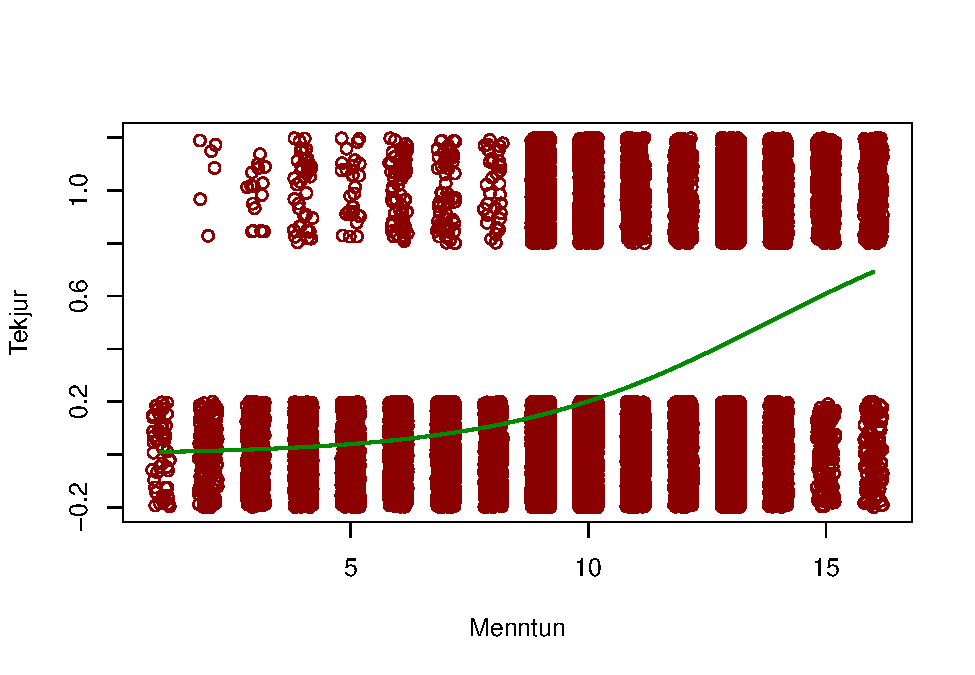
\includegraphics{timaglosur_files/figure-latex/unnamed-chunk-8-1.pdf}

Og loks getum við skoðað sennileikahlutfallsprófið fyrir lokalíkanið okkar.

\begin{Shaded}
\begin{Highlighting}[]
\KeywordTok{lrtest}\NormalTok{(likan1)}
\end{Highlighting}
\end{Shaded}

\begin{verbatim}
## Likelihood ratio test
## 
## Model 1: income ~ sex + age + education_num
## Model 2: income ~ 1
##   #Df LogLik Df  Chisq Pr(>Chisq)    
## 1   4 -14359                         
## 2   1 -17974 -3 7229.8  < 2.2e-16 ***
## ---
## Signif. codes:  0 '***' 0.001 '**' 0.01 '*' 0.05 '.' 0.1 ' ' 1
\end{verbatim}

\hypertarget{uxfeuxe1ttagreining}{%
\chapter{Þáttagreining}\label{uxfeuxe1ttagreining}}

Við notum þáttagreiningu þegar við viljum vita hversu margar hugsmíðar eru metnar með safni mælibreyta, hvaða hugsmíðar þetta kunna að vera án þess að vera kominn á þann stað að geta prófað ákveðnar tilgátur um orsakatengsl milli hugsmíðanna (bls. 20).

Algengt er að þáttagreining sé notuð til að koma auga á helstu hugsmíðar sem þarf til að gera grein fyrir innan tiltekins fræðasviðs (bls. 20)

Annað mikilvægt notagildi þáttagreiningar er að hjálpa til við þróun mælitækja til að leggja mat á hugsmíðar (bls. 22)

\hypertarget{markmiuxf0-uxfeuxe1ttagreiningar-og-lykilhugtuxf6k}{%
\section{Markmið þáttagreiningar og lykilhugtök}\label{markmiuxf0-uxfeuxe1ttagreiningar-og-lykilhugtuxf6k}}

Þáttagreining er aðferð til að ákvarða fjölda einstakra hugsmíða sem þarf til að gera grein fyrir mynstri fylgni milli mismunandi mælinga. Þetta má einnig setja fram á þann hátt að þáttagreiningu sé beitt til að ákvarða fjölda eintakra hugsmíða sem metnar eru með setti mælinga.

Þættir (eða common factors) eru undirliggjand/ómældar hugsmíðir sem gengið er út frá að geri grein fyrir fylgni milli breyta í gagnasafninu.

Þegar þáttagreining er framkvæmd fáum við líka upplýsingar sem hjálpa til við túlkun þáttanna og eðli þeirra. Þar ber fyrst að nefna þáttahleðslur (factor loadings) sem segja til um styrkleika og stefnu tengsla milli mælinga og undirliggjandi þáttar.

Mikilvæg hugtök:

\begin{itemize}
\tightlist
\item
  mældar breytur (measured variables)
\item
  safn mælibreyta (battery)
\item
  þáttur (common factor eða latent variable)
\item
  einstakir þættir (unique factors)

  \begin{itemize}
  \tightlist
  \item
    sértækur þáttur (specific factor)
  \item
    mælivilla (measurement error)
  \end{itemize}
\item
  Þáttaskýring (communality): Hlutfall dreifni sem er skýrð af almennu þáttunum (common factors). Eru reiknaðar með því að leggja saman hleðstlur ákveðinnar breytu í öðru veldi yfir þáttalausnina. Segir til um hversu mikið lausnin í heild sinni skýrir af dreifingu viðkomandi breytu.
\item
  Eigingildi (eigenvalue): Summa hleðsla sem búið er að setja í annað veldi fyrir tiltekinn þátt - segir til um hversu mikið af dreifni er skýrð af hverjum einstökum þætti þáttalausnarinnar. Oft notað til að ákvaða hversu marga þætti á að draga út úr gagnasafni fyrir þáttalausnina.
\end{itemize}

Formlega séð er þáttur skilgreindur sem ómæld hugsmíð sem hefur línuleg áhrif á meira en eina mælda breytu í safni mælibreyta. Á ensku eru þættir kallaðir common factors þar sem þeir eru sameiginlegir fyrir meira en eina breytu. Ennfremur er módelið skilgreint þannig að um verður að ræða mun færri þætti heldur en mældar breytur er til staðar í gagnasafninu. Þetta kemur til vegna þess að gengið er út frá þeirri forsíðu að fylgnistuðlar milli breyta í gagnasafni sem eru ekki núll, koma til vegna þess að báðar breyturnar (það er, þær sem mælast með fylgni sín á milli) eru undir áhrifum frá sömu undirliggjandi breytunni.

Einstakir þættir eru ómælanlegar uppsprettur línulegra áhrif á hverja einstaka breytu í gagnasafninu. Samkvæmt líkani þáttagreiningar standa einstakir þættir fyrir það skor mældrar breytu sem er ekki skýrt af þáttum líkansins. Þar sem einstakir þættir hafa aðeins áhrif á stakar mældar breytur í gagnasafninu og tengjast ekki hvor öðrum þá geta einstakir þættir ekki skýrt fylgni milli mældra breyta. Einstakir þættir skiptast í tvennt: Specific factor og mælivillu. Specific þátturinn vísar til kerfisbundinna áhrifa sem aðeins hafa áhrif á þessa tilteknu mældu breytu - þess vegna koma þessir þættir fram aftur og aftur í mælingum og hafa ekki áhrif á áreiðanleika mældrar breytu. Sterkir specific þættir benda til þess að mælingarnar eru undir miklum áhrifum hugsmíða sem þær áttu ekki að mæla. Hér er tekið dæmi um bjaga í orðalagi spurningar í mælitæki sem veðrur til þess að ýtt er undir líkurnar á ákveðnu svari hjá þátttakendum.

Mælivilla eru handahófskennd áhrif á einstaka mælda breytu. Þar sem áhrif hennar eru handahófskennd þá mun hún hafa áhrif á áreiðanleika mælinga í þáttagreiningu - ef um er að ræða sterka mælivillu þá mun áreiðanleiki mælinganna líða fyrir það. Dæmi um slíkt gæti verið spurning í spurningalista sem orðuð er á tvíræðan hátt þannig að svarendur gætu valið eitt svar á einum tímapunkti en annað svar síðar, allt eftir því hver ástand svaranda er þegar spurningin er lögð fyrir og við hvaða tilefni spurningin er lögð fyrir.

Horfa má á deifni í þáttagreiningu út frá eftirfarandi einföldu formúlum sem segja til um hvernig má skipta niður dreifni mældra breyta:

\begin{enumerate}
\def\labelenumi{\arabic{enumi})}
\tightlist
\item
  Mæld dreifni = sameiginleg dreifni + einstök dreifni
\item
  einstök dreifni = sértæk dreifni + villudreifni
\item
  þáttaskýring(1) = sameiginleg dreifni/mæld dreifni
\item
  þáttaskýring(1) = 1-(einstök dreifni/mæld dreifni)
\item
  Áreiðanleiki(2) = (sameiginleg dreifni+sértæk dreifni)/mæld dreifni
\item
  Áreiðanleiki(2) = 1-(villudreifni/mæld dreifni)
\end{enumerate}

\hypertarget{samdreifni--og-fylgnifylki}{%
\section{Samdreifni- og fylgnifylki}\label{samdreifni--og-fylgnifylki}}

Grundvöllur þáttagreiningar er samdreifnifylki (covariance matrix) en þar má sjá samdreifni allar breyta gagnasafnsins á móti hver annarri. Samdreifni skilgreinum við sem línulegt samband tveggja breyta sem er gefið upp á kvarða breytanna sjálfra. Samdreifni í úrtakinu segir okkur að hvaða marki tvær breytur breytast sameiginlega (eru tengdar) í þýðinu.

Formúlan fyrir samdreifni í úrtaki er eftirfarandi:
\(COV_{XY} = s_{xy} = \frac{\sum\limits_{i=1}^{n}{(X_{i}-\bar{X})(Y_{i}-\bar{Y})} }{n-1}\)

Þarna sjáum við að grunnurinn að baki því að skoða samdreifni er að við skoðum að hvaða marki hver mæling á X og samsvarandi mæling á Y víkur frá meðalgildi hvorrar breytu fyrir sig. Þetta er gert fyrir hvert tilvik í gagnasafninu, þau lögð saman og loks deilt með fjölda í úrtaki, mínus 1. Ef samdreifni breytu er reiknuð fyrir sjálfa sig þá má sýna fram á að það er í raun dreifni viðkomandi breytu. Þess vegna er skálína samdreifnifylkis alltaf til marks um dreifni viðkomandi breytu.

Samdreifni hefur engin mörk og getur bæði verið jákvæð eða neikvæð. Ef samdreifni er jákvæð er það til marks um að há gildi á annarri breytunni hafa tilhneigingu til að tengjast háum gildum á hinni breytunni. Neikvæði samdreifni merkir að há gildi á annarri breytunni tengjast að jafnaði lægri gildum á hinni breytunni. Ef samdreifnin er núll þá eru engin línuleg tengsl til staðar milli breytanna - það þýðir ekki að það séu engin tengsl, bara að það séu ekki línuleg tengsl.

Þar sem erfitt getur verið að túlka samdreifni þá er oft búin til stöðluð útgáfa af honum. Ef við tökum samdreifni og stöðlum hana þá fáum við fylgni. Með öðrum orðum er fylgni stöðluð samdreifni tveggja breyta.

\(r_{xy}=\frac{COV_{XY}}{s_{x}s_{y} }\)

Eins og sést er kjarni fylgninnar, styrkleiki hennar og stefna bæði tilkomin vegna samdreifninnar.

\hypertarget{duxe6mi-1}{%
\subsection{Dæmi}\label{duxe6mi-1}}

Í töflu \ref{tab:fylgnifylki} má sjá fylgnifylki fyrir gagnasett um hvaða þættir skipta mestu máli þegar fólk kaupir sér bjór. Í gagnasafninu eru alls níu breytur en sjö þeirra voru notaðar til að mæla eiginleika bjórs. Þessar sjö breytur voru:

\begin{itemize}
\tightlist
\item
  verð bjórsins
\item
  stærð
\item
  alkóhólsinnihald
\item
  orðspor bjórsins
\item
  liturinn
\item
  lyktin af bjórnum
\item
  bragðið
\end{itemize}

Hver og einn svarandi mat þessar breytur á hundrað punkta kvarða hversu mikilvægir honum þótti þær þegar komið væri að því að versla sex dósir af bjór.

\begin{table}

\caption{\label{tab:fylgnifylki}Fylgnifylki fyrir mat á mikilvægi eiginleika bjórs þegar ákvörðun er tekin um kaup.}
\centering
\begin{tabular}[t]{l|r|r|r|r|r|r|r}
\hline
  & COST & SIZE & ALCOHOL & REPUTAT & COLOR & AROMA & TASTE\\
\hline
COST & 1.00 & 0.84 & 0.78 & -0.39 & -0.03 & -0.05 & -0.11\\
\hline
SIZE & 0.84 & 1.00 & 0.91 & -0.37 & 0.10 & 0.10 & -0.05\\
\hline
ALCOHOL & 0.78 & 0.91 & 1.00 & -0.43 & -0.02 & 0.04 & -0.07\\
\hline
REPUTAT & -0.39 & -0.37 & -0.43 & 1.00 & -0.36 & -0.44 & -0.43\\
\hline
COLOR & -0.03 & 0.10 & -0.02 & -0.36 & 1.00 & 0.91 & 0.91\\
\hline
AROMA & -0.05 & 0.10 & 0.04 & -0.44 & 0.91 & 1.00 & 0.87\\
\hline
TASTE & -0.11 & -0.05 & -0.07 & -0.43 & 0.91 & 0.87 & 1.00\\
\hline
\end{tabular}
\end{table}

Til þess að gögn henti fyrir þáttagreiningu er mikilvægt að dreifing sé til staðar í fylgnifylkinu, það er, bæði sé um að ræða háar tölur (neikvæðar og jákvæðar) en einnig að fyrir hendi séu gildi sem eru núll eða nærri núlli. Ef þetta kemur fram í fylgnifylkinu þá er það til marks um að fyrir hendi séu undirliggjandi þættir sem hafa áhrif á vissar breytur en ekki aðrar og að milli þessara þátta sé takmörkuð eða engin fylgni.

\hypertarget{myndruxe6n-framsetning-uxfeuxe1ttagreiningar}{%
\section{Myndræn framsetning þáttagreiningar}\label{myndruxe6n-framsetning-uxfeuxe1ttagreiningar}}

Þegar við setjum myndrænt fram niðurstöður þáttagreiningu þá er það gert samkvæmt ákveðnum reglum. Dæmi um það má sjá á mynd \ref{fig:thatt1} þar sem búið er að þáttagreina bjórgagnasafnið með tveimur undirliggjandi þáttum. Á þessari mynd er ennfremur búið að lita þáttahleðslurnar með grænu eða rauðu eftir því hvort um er að ræða jákvæðar eða neikvæðar hleðslur á þættina.

Mikilvægustu þættirnir eru þó eftirfarandi:

\begin{itemize}
\tightlist
\item
  Þættir eru teiknaðir sem hringir
\item
  Mældar breytur eru teiknaðir sem ferhyrningar eða ferningar
\item
  Línuleg áhrif eru táknuð með örvum (með einum örvarenda) sem liggja frá viðkomandi þætti og í áttina að mældu breytunni sem er undir áhrifum frá viðkomandi þætti
\item
  Línuleg tengsl á borð við fylgni eru táknum með tvöföldum örvum
\item
  Ef um er að ræða tvöfalda ör sem fer frá tiltekinni breytu í sjálfa sig, þá er um að ræða dreifni viðkomandi breytu.
\item
  Tengsl breyta (hvort sem þau eru í ákveðna átt eða ekki) eru táknuð með því að skrifa tölugildið við nærri viðkomandi tengslum
\item
  Á myndina vantar einstöku þættina sem hafa áhrif á hverja mælda breytu en þeir eru jafnan táknaðir sem hringir fyrir neðan mældu breyturnar, einn fyrir hverja mælda breytu, sem hefur tengslin 1 við hverja breytu en enga fylgni sín á milli.
\end{itemize}

Hér er mikilvægt að taka eftir því að gert er ráð fyrir því að engin fylgni sé milli þáttanna tveggja sem sést á því að engin ör liggur milli þeirra tveggja. Þetta er kallað hornskökk þáttagreining (orthogonal factor analysis) og er algeng forsenda sem er gefin í þáttagreiningu. Fjallað verður betur um hana síðar.

Einnig er mikilvægt að benda á að um er að ræða tvo þætti en það er eitthvað sem rannsakandi hefur ákveðið að gera á grunni þáttagreiningarinnar. Það er, fjöldi þátta sem er dreginn út úr gagnasafninu er eitthvað sem rannsakandi ákveður og byggir þá ákvörðun sína á ýmsum gögnum og niðurstöðum sem fást úr þáttagreiningunni sjálfri.

\hypertarget{formuxfalur-uxfeuxe1ttagreiningar}{%
\section{Formúlur þáttagreiningar}\label{formuxfalur-uxfeuxe1ttagreiningar}}

Gott er að skoða helstu formúlu þáttagreiningar til að þekkja betur aðferðina og á hverju hún byggir. Yfirleitt er er þáttagreiningarlíkanið sett fram á formi fylkjareiknings.

\(P = \Lambda \Phi \Lambda^{T}+D_{\Psi}\)

Hérna þýðir P fylgnifylki í þýðinu fyrir mældar breytur í tilteknu safni mældra breyta sem við höfum áhuga á. Þetta fylgnifylki fæst með því að setja saman:

\begin{itemize}
\tightlist
\item
  fylkið Lambda, sem er fylki fyrir þáttahleðslur þáttalíkansins

  \begin{itemize}
  \tightlist
  \item
    segir til um styrk og stefnu tengslanna milli þáttanna og mældu breytanna
  \end{itemize}
\item
  fylkið Lambda T er sama fylkið og áður (það er, fyrir þáttahleðslur) nema búið er að snúa því þannig að það sem áður voru dálkar eru nú raðir og það sem áður voru raðir eru nú dálkar
\item
  fylkið fí er fylgnifylki milli þáttanna sem við erum að vinna með

  \begin{itemize}
  \tightlist
  \item
    þegar unnið er með hornrétta þáttagreiningu þá getum við sleppt þessu fylki úr útreikningunum þar sem gengið er út frá því að engin fylgni sé milli þáttanna: \(P = \Lambda\Lambda^{T}+D_{\Psi}\)
  \end{itemize}
\item
  síðasta fylkið í formúlunni er D-psi en það stendur fyrir samdreifnifylki milli einstöku þáttanna. Þess vegna verður skálína fylkisins dreifni einstöku þáttanna en aðrir hlutar fylkisins eru núll þar sem ekki er gert ráð fyrir fylgni milli einstöku þáttanna.

  \begin{itemize}
  \tightlist
  \item
    ennfremur, þar sem gert er ráð fyrir að mældu breyturnar hafi verið staðlaðar með corrlation structure modelinu, þá táknar skálínan í raun hlutfall dreifninnar í hverri mældri breytu sem skýrð er með einstöku þáttunum.
  \end{itemize}
\end{itemize}

Þegar við tökum þetta saman þá þýðir þetta að ef við erum með hornrétta þáttagreiningu, þá teljum við okkur geta smíðað fylgnifylki breytanna í þýði með því að margfalda þáttahleðslufylkið með snúnu útgáfu af sjálfu sér og leggja við það samdreifnifylki einstakra þátta. Ef um væri að ræða hornskakkan snúning þá myndum við margfalda fyrri hluta formúlunnar með fylgnifylki þáttanna í líkaninu.

\hypertarget{annauxf0-duxe6mi}{%
\subsection{Annað dæmi}\label{annauxf0-duxe6mi}}

Nú ætlum við að skoða annað dæmi. Við erum með gagnasafn yfir alla leikmenn sem hafa á einhverjum tímapunkti spilað með Boston Celtics í NBA deildinni í körfubolta. Við hreinsum aðeins til og veljum aðeins þá sem spiluðu fleiri en 50 leiki með liðinu. Einnig, þar sem varin skot voru fyrst talin tímabilið 1973 - 74 þá ætlum við aðeins að skoða leikmenn sem hófu að spila fyrir liðið eftir það tímabil. Við viljum skoða hvort hægt sé að finna undirliggjandi víddir fyrir hefðbundnar tölfræðimælingar á leikmönnum liðsins. Um er að ræða eftirfarandi mælibreytur:

\begin{itemize}
\tightlist
\item
  Stolnir boltar
\item
  Varin skot
\item
  Tapaðir boltar
\item
  Villur
\item
  Skotnýtingu
\item
  Þriggja stiga skotnýtingu
\item
  Vítaskotnýtingu
\item
  Mínútur spilaðar að meðaltali í leik
\item
  Skoruð stig að meðaltali í leik
\item
  Fráköst að meðaltali í leik
\item
  Stoðsendingar að meðaltali í leik
\end{itemize}

\begin{table}

\caption{\label{tab:BCfylgni}Fylgnifylki fyrir leikmenn Boston Celtics frá 1974.}
\centering
\begin{tabular}[t]{l|r|r|r|r|r|r|r|r|r|r|r}
\hline
  & stol & vskot & tapb & vill & sknyt & sknyt3 & sknyV & min & stig & frak & stods\\
\hline
stol & 1.00 & 0.54 & 0.93 & 0.85 & 0.16 & 0.11 & 0.16 & 0.58 & 0.60 & 0.45 & 0.49\\
\hline
vskot & 0.54 & 1.00 & 0.74 & 0.83 & 0.39 & -0.14 & 0.04 & 0.35 & 0.43 & 0.61 & 0.04\\
\hline
tapb & 0.93 & 0.74 & 1.00 & 0.94 & 0.27 & 0.01 & 0.12 & 0.56 & 0.63 & 0.54 & 0.43\\
\hline
vill & 0.85 & 0.83 & 0.94 & 1.00 & 0.36 & -0.04 & 0.08 & 0.52 & 0.56 & 0.60 & 0.26\\
\hline
sknyt & 0.16 & 0.39 & 0.27 & 0.36 & 1.00 & -0.29 & -0.03 & 0.20 & 0.23 & 0.48 & -0.03\\
\hline
sknyt3 & 0.11 & -0.14 & 0.01 & -0.04 & -0.29 & 1.00 & 0.30 & 0.25 & 0.23 & -0.11 & 0.24\\
\hline
sknyV & 0.16 & 0.04 & 0.12 & 0.08 & -0.03 & 0.30 & 1.00 & 0.36 & 0.44 & 0.07 & 0.31\\
\hline
min & 0.58 & 0.35 & 0.56 & 0.52 & 0.20 & 0.25 & 0.36 & 1.00 & 0.89 & 0.62 & 0.65\\
\hline
stig & 0.60 & 0.43 & 0.63 & 0.56 & 0.23 & 0.23 & 0.44 & 0.89 & 1.00 & 0.61 & 0.57\\
\hline
frak & 0.45 & 0.61 & 0.54 & 0.60 & 0.48 & -0.11 & 0.07 & 0.62 & 0.61 & 1.00 & 0.11\\
\hline
stods & 0.49 & 0.04 & 0.43 & 0.26 & -0.03 & 0.24 & 0.31 & 0.65 & 0.57 & 0.11 & 1.00\\
\hline
\end{tabular}
\end{table}

Út frá þessum niðurstöðum getum við prófað okkur áfram með að búa til þáttalíkan fyrir þessi gögn. Án þess að leggja mikla hugsun í þetta þá gerum við þriggja þátta líkan. Út frá þessu líkani þá getum við reiknað okkur í gegnum formúluna: \(P = \Lambda \Phi \Lambda^{T}+D_{\Psi}\)

Með því ætlum við að skoða hversu nálægt upprunalega fylgnifylkinu við komumst með því að endurgera það út frá niðurstöðum þáttagreiningarinnar. Fyrsta skrefið er að finna lambda fylkið, sem er fyrir þáttahleðslurnar. Það má sjá í töflu \ref{tab:lambdafylki}. Í töflunni sjáum við allar þáttahleðslur fyrir hverja og eina mælda breytu fyrir hvern og einn þátt.

\begin{table}

\caption{\label{tab:lambdafylki}Lambda fylki}
\centering
\begin{tabular}[t]{l|r|r|r}
\hline
  & Factor1 & Factor2 & Factor3\\
\hline
stol & 0.89 & -0.24 & -0.31\\
\hline
vskot & 0.69 & -0.39 & 0.49\\
\hline
tapb & 0.92 & -0.33 & -0.08\\
\hline
vill & 0.89 & -0.38 & 0.13\\
\hline
sknyt & 0.29 & -0.09 & 0.41\\
\hline
sknyt3 & 0.11 & 0.30 & -0.27\\
\hline
sknyV & 0.24 & 0.32 & -0.09\\
\hline
min & 0.81 & 0.56 & 0.04\\
\hline
stig & 0.81 & 0.41 & 0.04\\
\hline
frak & 0.66 & 0.12 & 0.44\\
\hline
stods & 0.54 & 0.39 & -0.42\\
\hline
\end{tabular}
\end{table}

Næsta skref er að snúa lambdafylkinu. Það er einfalt mál og má sjá í \ref{tab:snuidlambdafylki}.

\begin{table}

\caption{\label{tab:snuidlambdafylki}Lambda fylki}
\centering
\begin{tabular}[t]{l|r|r|r|r|r|r|r|r|r|r|r}
\hline
  & stol & vskot & tapb & vill & sknyt & sknyt3 & sknyV & min & stig & frak & stods\\
\hline
Factor1 & 0.89 & 0.69 & 0.92 & 0.89 & 0.29 & 0.11 & 0.24 & 0.81 & 0.81 & 0.66 & 0.54\\
\hline
Factor2 & -0.24 & -0.39 & -0.33 & -0.38 & -0.09 & 0.30 & 0.32 & 0.56 & 0.41 & 0.12 & 0.39\\
\hline
Factor3 & -0.31 & 0.49 & -0.08 & 0.13 & 0.41 & -0.27 & -0.09 & 0.04 & 0.04 & 0.44 & -0.42\\
\hline
\end{tabular}
\end{table}

Þessi tvö fylki eru margfölduð saman (eins og gera má í fylkjareikningi) og loks er d-psi fylkinu bætt við, sem sjá má í \ref{tab:dpsifylki}. Í þessu dæmi erum við með að vinna með ótengda þætti og því getum við slepp fí-fylkinu úr greiningunni.

\begin{table}

\caption{\label{tab:dpsifylki}D-psi fylki}
\centering
\begin{tabular}[t]{r|r|r|r|r|r|r|r|r|r|r}
\hline
1 & 2 & 3 & 4 & 5 & 6 & 7 & 8 & 9 & 10 & 11\\
\hline
0.05 & 0.00 & 0.00 & 0.00 & 0.00 & 0.00 & 0.00 & 0.00 & 0.00 & 0.00 & 0.00\\
\hline
0.00 & 0.13 & 0.00 & 0.00 & 0.00 & 0.00 & 0.00 & 0.00 & 0.00 & 0.00 & 0.00\\
\hline
0.00 & 0.00 & 0.03 & 0.00 & 0.00 & 0.00 & 0.00 & 0.00 & 0.00 & 0.00 & 0.00\\
\hline
0.00 & 0.00 & 0.00 & 0.04 & 0.00 & 0.00 & 0.00 & 0.00 & 0.00 & 0.00 & 0.00\\
\hline
0.00 & 0.00 & 0.00 & 0.00 & 0.74 & 0.00 & 0.00 & 0.00 & 0.00 & 0.00 & 0.00\\
\hline
0.00 & 0.00 & 0.00 & 0.00 & 0.00 & 0.83 & 0.00 & 0.00 & 0.00 & 0.00 & 0.00\\
\hline
0.00 & 0.00 & 0.00 & 0.00 & 0.00 & 0.00 & 0.84 & 0.00 & 0.00 & 0.00 & 0.00\\
\hline
0.00 & 0.00 & 0.00 & 0.00 & 0.00 & 0.00 & 0.00 & 0.02 & 0.00 & 0.00 & 0.00\\
\hline
0.00 & 0.00 & 0.00 & 0.00 & 0.00 & 0.00 & 0.00 & 0.00 & 0.17 & 0.00 & 0.00\\
\hline
0.00 & 0.00 & 0.00 & 0.00 & 0.00 & 0.00 & 0.00 & 0.00 & 0.00 & 0.35 & 0.00\\
\hline
0.00 & 0.00 & 0.00 & 0.00 & 0.00 & 0.00 & 0.00 & 0.00 & 0.00 & 0.00 & 0.38\\
\hline
\end{tabular}
\end{table}

Með þessar upplýsingar í farteskinu getum við nú reiknað okkar útgáfu af fylgnifylki þýðisins. Það má sjá í töflu \ref{tab:popcorrmatrix}. Það getum við svo borið saman við upprunalega fylgnifylkið okkar.

\begin{table}

\caption{\label{tab:popcorrmatrix}Fylgnifylki þýðisins út frá niðurstöðum þáttagreiningar}
\centering
\begin{tabular}[t]{l|r|r|r|r|r|r|r|r|r|r|r}
\hline
  & stol & vskot & tapb & vill & sknyt & sknyt3 & sknyV & min & stig & frak & stods\\
\hline
stol & 1.00 & 0.56 & 0.93 & 0.85 & 0.16 & 0.11 & 0.16 & 0.58 & 0.61 & 0.43 & 0.52\\
\hline
vskot & 0.56 & 1.00 & 0.73 & 0.83 & 0.44 & -0.17 & 0.00 & 0.36 & 0.42 & 0.63 & 0.01\\
\hline
tapb & 0.93 & 0.73 & 1.00 & 0.94 & 0.27 & 0.02 & 0.12 & 0.56 & 0.61 & 0.54 & 0.41\\
\hline
vill & 0.85 & 0.83 & 0.94 & 1.00 & 0.35 & -0.05 & 0.08 & 0.52 & 0.58 & 0.61 & 0.29\\
\hline
sknyt & 0.16 & 0.44 & 0.27 & 0.35 & 1.00 & -0.10 & 0.01 & 0.20 & 0.22 & 0.36 & -0.05\\
\hline
sknyt3 & 0.11 & -0.17 & 0.02 & -0.05 & -0.10 & 1.00 & 0.14 & 0.25 & 0.20 & -0.01 & 0.29\\
\hline
sknyV & 0.16 & 0.00 & 0.12 & 0.08 & 0.01 & 0.14 & 1.00 & 0.37 & 0.32 & 0.16 & 0.29\\
\hline
min & 0.58 & 0.36 & 0.56 & 0.52 & 0.20 & 0.25 & 0.37 & 1.00 & 0.89 & 0.62 & 0.65\\
\hline
stig & 0.61 & 0.42 & 0.61 & 0.58 & 0.22 & 0.20 & 0.32 & 0.89 & 1.00 & 0.61 & 0.58\\
\hline
frak & 0.43 & 0.63 & 0.54 & 0.61 & 0.36 & -0.01 & 0.16 & 0.62 & 0.61 & 1.00 & 0.22\\
\hline
stods & 0.52 & 0.01 & 0.41 & 0.29 & -0.05 & 0.29 & 0.29 & 0.65 & 0.58 & 0.22 & 1.00\\
\hline
\end{tabular}
\end{table}

Í töflu \ref{tab:popcorrmatrix} er samanburður við upprunalega fylgnifylkið (fyrir ofan skálínu) og fylgnifylkið sem kom út úr þáttagreiningunni (fyrir neðan skálínu). Eins og sjá má eru niðurstöðurnar nokkurn veginn þær sömu, þó mögulega væri hægt að bæta mátgæðin enn frekar með því að minnka muninn milli upprunalega fylgnifylkisins og þess sem var gert út frá þáttagreiningu.

\begin{table}

\caption{\label{tab:popcorrmatrix2}Tvö fylgnifylki; yfir skálínunni er upprunalega fylgnifylkið, undir skálínunni er fylgnifylgi út frá þáttagreiningunni}
\centering
\begin{tabular}[t]{l|r|r|r|r|r|r|r|r|r|r|r}
\hline
  & stol & vskot & tapb & vill & sknyt & sknyt3 & sknyV & min & stig & frak & stods\\
\hline
stol & 1.00 & 0.54 & 0.93 & 0.85 & 0.16 & 0.11 & 0.16 & 0.58 & 0.60 & 0.45 & 0.49\\
\hline
vskot & 0.56 & 1.00 & 0.74 & 0.83 & 0.39 & -0.14 & 0.04 & 0.35 & 0.43 & 0.61 & 0.04\\
\hline
tapb & 0.93 & 0.73 & 1.00 & 0.94 & 0.27 & 0.01 & 0.12 & 0.56 & 0.63 & 0.54 & 0.43\\
\hline
vill & 0.85 & 0.83 & 0.94 & 1.00 & 0.36 & -0.04 & 0.08 & 0.52 & 0.56 & 0.60 & 0.26\\
\hline
sknyt & 0.16 & 0.44 & 0.27 & 0.35 & 1.00 & -0.29 & -0.03 & 0.20 & 0.23 & 0.48 & -0.03\\
\hline
sknyt3 & 0.11 & -0.17 & 0.02 & -0.05 & -0.10 & 1.00 & 0.30 & 0.25 & 0.23 & -0.11 & 0.24\\
\hline
sknyV & 0.16 & 0.00 & 0.12 & 0.08 & 0.01 & 0.14 & 1.00 & 0.36 & 0.44 & 0.07 & 0.31\\
\hline
min & 0.58 & 0.36 & 0.56 & 0.52 & 0.20 & 0.25 & 0.37 & 1.00 & 0.89 & 0.62 & 0.65\\
\hline
stig & 0.61 & 0.42 & 0.61 & 0.58 & 0.22 & 0.20 & 0.32 & 0.89 & 1.00 & 0.61 & 0.57\\
\hline
frak & 0.43 & 0.63 & 0.54 & 0.61 & 0.36 & -0.01 & 0.16 & 0.62 & 0.61 & 1.00 & 0.11\\
\hline
stods & 0.52 & 0.01 & 0.41 & 0.29 & -0.05 & 0.29 & 0.29 & 0.65 & 0.58 & 0.22 & 1.00\\
\hline
\end{tabular}
\end{table}

\hypertarget{uxed-hvauxf0-notum-viuxf0-uxfeuxe1ttagreiningu}{%
\section{Í hvað notum við þáttagreiningu?}\label{uxed-hvauxf0-notum-viuxf0-uxfeuxe1ttagreiningu}}

Tvennskonar tilgangur

\hypertarget{koma-auga-uxe1-hugsmuxeduxf0ar-innan-uxe1kveuxf0ins-sviuxf0s-construct-identification.}{%
\subsection{1. Koma auga á hugsmíðar innan ákveðins sviðs (construct identification).}\label{koma-auga-uxe1-hugsmuxeduxf0ar-innan-uxe1kveuxf0ins-sviuxf0s-construct-identification.}}

Hægt að setja fram í fjórum skrefum:

\begin{enumerate}
\def\labelenumi{\arabic{enumi})}
\tightlist
\item
  Skilgreina fræðasviðið (define the domain);
\item
  Búa til eða finna mælibreytur;
\item
  Safna gögnum fyrir mælibreyturnar;
\item
  keyra þáttagreiningu til að ákvarða hvaða undirliggjandi breytur eru til staðar. Þetta eru þá undirliggjandi hugsmíðar sviðsins.
  Gott væri að taka dæmi.
\end{enumerate}

\begin{itemize}
\tightlist
\item
  Dæmi: Persónuleikaþættir -- þar komu fram fimm undirliggjandi þættir fyrir sviðið (sem var þá persónuleiki)
\end{itemize}

\hypertarget{vinna-viuxf0-smuxeduxf0i-muxe6lituxe6kja-uxed-suxe1lfruxe6uxf0i.}{%
\subsection{2. Vinna við smíði mælitækja í sálfræði.}\label{vinna-viuxf0-smuxeduxf0i-muxe6lituxe6kja-uxed-suxe1lfruxe6uxf0i.}}

\begin{enumerate}
\def\labelenumi{\arabic{enumi})}
\item
  Scale dimensionality -- hvaða víddir eru undirliggjandi viðkomandi kvarða. Oft eru sett saman mælitæki úr mörgum atriðum sem er ætlað að mæla eina undirliggjandi hugsmíð. Þáttagreining er mjög heppileg aðferð til að kanna þetta. Með því að keyra þáttagreiningu á mælingum með tilteknum kvarða þá má sjá hvort að um sé að ræða eina undirliggjandi vídd eða hvort víddirnar eru fleiri.
  DÆMI: Þankaþörf (need for cognition)
\item
  Þáttagreining veitir mikilvægar upplýsingar um mælifræðilega eiginleika spurningalistans -- atriði sem er sterklega undir áhrif frá þættinum sem hefur einnig sterk áhrif á önnur atriði listans sem er ætlað að mæla sömu hugsmíðina bendir sterklega til þess að atriðið sé raunverulega að ná utan um hugsmíðina sem því er ætlað að mæla.
\end{enumerate}

Að sama skapi: Atriði sem hleður lágt á þátt en þátturinn hefur sterk áhrif á önnur atriði sem eiga að mæla tiltekna hugsmíð er væntanlega légleg mæling á hugsmíðinni.

Ennfremur: Ef þegar mismunandi atriði eiga að mæla mismunandi hugsmíðar þá er hægt að nota þáttagreiningu til að meta áhrif allra hugsmíða á öll atriðin. Þannig er hægt að koma auga á atriði sem eru ekki hreinar mælingar á einum þætti -- það er þegar fleiri en einn þáttur hefur sterk tengsl við eitt atriði. Út frá þessum upplýsingum má hanna undirkvarða í mælitækinu -- þar sem aðeins eru valin atriði sem hlaða sterklega á einn þátt en taka út atriði sem hlaða á fleiri en einn þátt.

\hypertarget{forsendur-uxfeuxe1ttagreiningar}{%
\section{Forsendur þáttagreiningar}\label{forsendur-uxfeuxe1ttagreiningar}}

\hypertarget{eiginleikar-muxe6ldu-breytanna}{%
\subsection{Eiginleikar mældu breytanna:}\label{eiginleikar-muxe6ldu-breytanna}}

\begin{itemize}
\tightlist
\item
  Réttmæti þáttalausnarinnar veltur á því að mælibreyturnar séu lýsandi fyrir það svið sem þeim er ætlað að mæla.
\item
  Hversu margar breytur? Yfirleitt mælt með 3-5

  \begin{itemize}
  \tightlist
  \item
    Overdetermined er mikilvægt hugtak í þáttagreiningu sem merkir að mikilvægt er að huga vel að
    fjölda breyta fyrir hvern þátt á þann hátt að betra er að vera með fleiri en færri breytur fyrir
    hvern mældan þátt. Þannig er rétt fyrir rannsakanda sem ætlar sér að vera með fimm breytur fyrir
    tiltekinn þátt að vera með fleiri en fimm mældar breytur þegar rannsókninn er hönnuð.
  \end{itemize}
\item
  Gæði mældu breytanna -- FA virkar betur ef communalities fyrir breyturnar er hátt -- ein ástæða fyrir lágu communalities er há mælivilla (random error). Þannig að rétt er að vanda og hafa í huga best practices í spurningagerð.
\item
  Kvarði mælinga og dreifing -- interval level eða quasi-interval level

  \begin{itemize}
  \tightlist
  \item
    Ekki hægt að nota nafnbreytur eða raðbreytur
  \item
    Muna linearity
  \item
    Ef við notum Maximum likelihood þá er líka forsenda að breyturnar séu normaldreifðar
  \end{itemize}
\end{itemize}

\hypertarget{eiginleikar-uxfartaksins}{%
\subsection{Eiginleikar úrtaksins}\label{eiginleikar-uxfartaksins}}

\begin{itemize}
\tightlist
\item
  Hversu stórt þarf úrtakið að vera?

  \begin{itemize}
  \tightlist
  \item
    Allskonar þumalfingursreglur um þetta -- stundum miðað við hlutfall milli mældra breyta og þátttakenda (til dæmis, fimm þátttakendur fyrir hverja breytu)
  \item
    Flestar þessara reglna eru rugl og geta annað hvort valdið því að úrtakið verður ekki nógu stórt til að styðja ályktunartöku á grundvelli þáttagreiningarinnar eða að það verða stærra en þarf og þar með er búið að eyða fjármunum og tíma í óþarfa söfnun gagna
  \item
    Úrtaksstærð fyrir þáttagreiningu byggir á sömu grundvallarforsendum og úrtaksstærð í öllum öðrum rannsóknum sem eru gerðar í félagsvísindum.

    \begin{itemize}
    \tightlist
    \item
      Nauðsynleg úrtaksstærð veltur á þeim mælingum sem á að gera í úrtakinu -- sem setur rannsakendur í ákveðinn vanda: Hvernig er hægt að vita hvernig niðurstöðurnar verða þegar ekki er búið að gera rannsóknina?
    \item
      Þá verður að gera prófanir eða nákvæmar forskoðanir til að skipuleggja gagnasöfnunina og
      reyna að leggja mat á hversu stórt úrtak þarf líklega til að fá fram nægilega nákvæmar
      niðurstöður. Í það minnsta þarf rannsakandi að reyna eins og kostur er að
    \item
      Nokkrar sviðsmyndir:

      \begin{itemize}
      \tightlist
      \item
        Optimal conditions: Há communalities (.7) og þættir allir overdetermined (3 -- 5
        mælibreytur per þátt) -\textgreater{} oft dugar úrtak af stærðinni 100

        \begin{itemize}
        \tightlist
        \item
          Very well conditioned data - \textgreater{} hugsanlega dugar úrtak af stærðinni 50
        \end{itemize}
      \item
        Moderately good conditions: Communalities milli .4 og .7 og að minnsta kosti 3 breytur
        mældar fyrir hvern þátt -\textgreater{} Þá þarf að lágmarki úrtak af stærðinni 200
      \item
        Poor conditions: Communalities lægri en .4 og sumir þættir aðeins með tvær breytur sem
        hlaða á þá -\textgreater{} Að lágmarki þarf úrtak af stærðinni 400 en hugsanlega myndi ekki einu sinni
        duga að hafa mjög stórt úrtak.
      \end{itemize}
    \end{itemize}
  \item
    Auðvitað ættu úrtök alltaf að vera lýsandi fyrir þann hóp sem er ætlast til að það muni lýsa -- höfundar segja að það sé í lagi að nota þægindaúrtak. En er það\ldots{}?
  \end{itemize}
\end{itemize}

``Convenience samples need not be a problem so long as the biases in the sample are not strongly related to the constructs of interest. Thus, although some university samples might not be appropriate for tests of particular cognitive abilities (e.g., a sample of this sort might be highly nonrepresentative of the population on cognitive abilities such as verbal ability), for other constructs, such as perceptual abilities, a student sample might not be appreciably different from the population as a whole. Hence, researchers should carefully consider the nature of their samples and their relations to the domains of interest. When there is reason to expect that biases may exist in the sample, the results of any factor analysis should always be interpreted with an awareness of how sample homogeneity might have contributed to the results (bls 27.)''

Í sjálfu sér er þetta hárrétt hjá höfundum bókarinnar -- en yfirleitt er fjarstæðukennt að ætlast til þess að rannsakendur geti mögulega skoða þessa eiginleika úrtaksins empirískt.

Umfjöllun höfunda um missing data er ábótavant. Til dæmis er aldrei viðeigandi að nota meðaltal sem gildi tilreiknunar fyrir gagnagöt, það bíður upp á bjaga í niðurstöðum. Áhugasömum stúdentum er bent á að kynna sér aðferð sem kallast multiple imputation. Það er aðferð sem byggir á því að gera líkan fyrir gagnagöt í gagnasafni þar sem nýttar eru upplýsingar allra annarra breyta til að búa til trúverðug gildi í stað þeirra sem vantar. Með því að nota MI er ennfremur stjórnað fyrir þann bjaga sem kann að koma fram á mati á dreifni þegar tilreiknun er beitt. Það er gert með því að búin eru til k-fjöldi gagnasafna sem öll eru með mismunandi tilreiknuðu gildi.

Besta bókin er: Flexible imputation of Missing data eftir Stef van Buuren. Svo má líka lesa eitthvað eftir Rubin en þær bækur eru jafnan frekar tæknilegar.

\hypertarget{leitandi-euxf0a-stauxf0festandi-uxfeuxe1ttagreining}{%
\section{Leitandi eða staðfestandi þáttagreining}\label{leitandi-euxf0a-stauxf0festandi-uxfeuxe1ttagreining}}

Hægt er að skipta þáttagreiningu í tvennt: Leitandi þáttagreiningu (Exploratory Factor Analysis, EFA) og staðfestandi þáttagreiningu (Confirmatory Factor Analysis; CFA). Þegar um er að ræða leitandi þáttagreiningu hefur rannsakandi ekki neina sérstaka hugmynd um hvaða undirliggjandi þáttabygging er til staðar og lætur kyltu ráða kasti. Þegar um er að ræða staðfestandi þáttagreiningu hefur rannsakandi ákveðnar hugmyndir eða tilgátur um sambandið milli breytanna og hvaða undirliggjandi víddir eru til staðar. Þessar tilgátur eru prófaðar með því gagnasafni sem rannsakandi hefur aðgang að og metið að hvaða marki gögnin og sambandið milli breytanna víkur frá tilgátum rannsakana.

\hypertarget{hvort-uxe1-auxf0-nota-leitandi-euxf0a-stauxf0festandi-uxfeuxe1ttagreiningu}{%
\subsection{Hvort á að nota leitandi eða staðfestandi þáttagreiningu?}\label{hvort-uxe1-auxf0-nota-leitandi-euxf0a-stauxf0festandi-uxfeuxe1ttagreiningu}}

Veltur að einhverju leyti á því hvort rannsakandi er með tilgátur um hvaða þættir eru til staðar, hvaða breytur hlaða á hvern þátt og hver eru tengslin milli þátta. Sérstaklega er mikilvægt að beita CFA þegar rannsakandi er með nokkur líkön -- þá er hægt að keyra CFA fyrir hvert líkan og meta hvert þeirra er með hæstu mátgæðin (fit). Mátgæti er til marks um hversu vel líkanið passar við undirliggjandi gögnin sem CFA er reiknað á. Það líkan sem er með hæst (eða best mátgæði) er þá það líkan sem rannsakandi heldur sig við. Hins vegar ef um er að ræða gríðarlegan fjölda módela sem öll koma til greina -- þá er að öllum líkindum betra að keyra EFA. Eins, ef rannsakandi hefur gjörsamlega enga hugmynd um hvaða mun koma út úr þáttagreiningunni.

\hypertarget{hver-er-munurinn-uxe1-uxfeuxe1ttagreiningu-og-meginhlutagreiningu-fa-vs-pca}{%
\section{Hver er munurinn á þáttagreiningu og meginhlutagreiningu (FA vs PCA)}\label{hver-er-munurinn-uxe1-uxfeuxe1ttagreiningu-og-meginhlutagreiningu-fa-vs-pca}}

Oft er gert ráð fyrir að PCA sé ákveðin tegund af FA -- en það er ekki rétt.

``PCA essentially involves a model in which a small set of principal components are constructed from the measured variables, and the ability of these components to predict the measured variables is assessed (as indexed by the principal component loadings) (bls. 32.).''

\hypertarget{uxfeuxe1ttagreining-1}{%
\subsection{Þáttagreining}\label{uxfeuxe1ttagreining-1}}

Helstu einkenni í samanburði við meginhlutagreiningu:

\begin{itemize}
\item
  Aðferð til að skilja strúktúr fylgni milli mældra breyta -- hver mæld breyta er línuleg samsetning undirliggjandi þáttarins og unique factor (specific factor og random error)
\item
  Hægt er að túlka þætti sem undirliggjandi breytur
\item
  Common factors eru latent constructs sem orsaka mælibreyturnar (samkvæmt kenningunni). Dreifni er skipt í common variance (dreifni sem kemur til vegna þáttanna) og unique variance (sem kemur til vegna áhrifa sem aðeins hafa áhrif á viðkomandi atriði)
\end{itemize}

\hypertarget{meginhlutagreining}{%
\subsection{Meginhlutagreining}\label{meginhlutagreining}}

Ef unnið er með stórt gagnasafn þar sem fylgni er milli breyta þá gerir meginhlutagreining okkur kleyft að taka saman breyturnar í safninu í færri meginhluta sem í sameiningu skýra megnið af dreifingunni í upprunalega gagnasafninu. Meginhlutarnir eru þá lýsandi (representative) breytur fyrir alla dreifni gagnasafnsins. Meginhlutagreining er tækni þar sem hægt er að búa til meginhlutana á grunni gagnasafnsins og nota þá í frekari greiningum. Meginhlutagreining er meðal annars notuð í vélrænu námi sem leitandi leið til að skoða gagnasafn og tengslin sem eru til staðar innan þess.

Meginhlutagreining eru notuð til að finna leið til að lýsa gögnunum út frá fáum víddum (low-dimensional representation) sem innihalda eins mikið af dreifni gagnasafnsins og hægt er. Hugmyndin er að hver og ein mæling (n) í gagnasafninu eigi sér stað í rými sem er með p-víddum en ekk allar þessara víddar eru jafn áhugaverðar. Meginhlutagreining leitar eftir fáum víddum sem eru eins áhugaverðar og mögulegt er. Í þessu samhengi vísar ``áhugaverðar'' til þess hversu mikið mælingarnar dreifast eftir hverri vídd. Hver vídd sem greiningin finnur er línuleg samsetning af p-einkennunum. Þannig að í meginhlutagreiningu er takmarkið altaf að reyna að skýra eins mikið af dreifingu gagnasafnsins með fáum meginhlutum. Það er svo gert með því að finna fyrsta meginhlutann í gögnunum sem skýrir eins mikið af dreifingu og hægt er og svo koll af kolli, út frá þeirri forsendu að meginhlutarnir séu hornréttir (orthogonal) miðað við hina meginhlutana, það er, engin fylgni er leyfð milli meginhlutanna en þeirra hlutverk er að safna saman allri dreifni og samdreifni gagnasafnsins.

Helstu einkenni meginhlutagreiningar í samanburði við þáttagreiningu:

\begin{itemize}
\item
  Hannað til að sjóða niður skor á breytusafni -- í sett af færri skorum (sem eru meginhlutarnir). Helsta takmarkið er að taka saman eins mikið og hægt er af dreifni mælibreytanna -- en ekki að skýra fylgni milli breytanna.
\item
  Ekki er hægt að túlka meginhlutana sem raunverulega latent hugtök -- þeir eru einungis til marks um hagkvæma aðferð til að ná utan um eins mikið af upplýsingum sem eru til staðar í mældu breytunum og hægt er.
\item
  Meginhlutar eru reiknaðir beint frá mælibreytunum og því innihalda þeir bæði common og unique variance.
\end{itemize}

\hypertarget{af-hverju-uxe6tti-meginhlutagreining-auxf0-vera-notuuxf0-frekar-en-uxfeuxe1ttagreining}{%
\subsection{Af hverju ætti meginhlutagreining að vera notuð frekar en þáttagreining?}\label{af-hverju-uxe6tti-meginhlutagreining-auxf0-vera-notuuxf0-frekar-en-uxfeuxe1ttagreining}}

Nefnd eru þrjú atriði sem oft eru rædd í samhengi við að PCA sé heppilegri aðferð miðað við FA:

\begin{enumerate}
\def\labelenumi{\arabic{enumi})}
\tightlist
\item
  PCA er einfaldari í útreikningi og þarf því ekki eins öflugar tölvur
\end{enumerate}

\begin{itemize}
\tightlist
\item
  Þetta á klárlega ekki við lengur
\end{itemize}

\begin{enumerate}
\def\labelenumi{\arabic{enumi})}
\setcounter{enumi}{1}
\tightlist
\item
  Niðurstöður PCA eru jafnan mjög svipaðar niðurstöðum FA á sama gagnasafni
\end{enumerate}

\begin{itemize}
\tightlist
\item
  Í ýmsum tilvikum er það ekki svo -- sérstaklega þegar communalities eru tiltölulega lág (.40 eða lægri) og fáar breytur hlaða á hvern þátt.
\item
  Þar sem þetta eru algengar aðstæður í rannsóknum félagsvísinda þá er munurinn milli aðferðanna algengari en halda mætti
\item
  Þegar forsendur FA halda -- þá eru niðurstöður FA nákvæmari en í PCA. Þegar forsendur PCA (presence of little unique variance) halda, þá eru niðurstöður PCA samt ekki nákvæmari heldur en FA.
\end{itemize}

\begin{enumerate}
\def\labelenumi{\arabic{enumi})}
\setcounter{enumi}{2}
\tightlist
\item
  Í EFA koma stundum fram Heywood cases (þar sem communality er 1 eða hærra en 1 -- conceptually implausible eða impossible estimates)
\end{enumerate}

\begin{itemize}
\tightlist
\item
  Mikilvægt er að halda því til haga að Heywood case koma fram þegar líkanið hefur verið misspecified (alvarlega) eða gögnin víkja alvarlega frá forsendum common factor líkansins.
\item
  Þess vegna má segja að Heywood case hafi ákveðið greiningargildi það er miklu betra að vita af þeim og geta þá gripið til viðeigandi aðgerða heldur en að vita ekki af þeim og PCA keyrir eins og ekkert hafi komið upp á. PCA leysir semsagt ekki þessi vandamál -- hún lítur bara framhjá þeim.
\end{itemize}

\begin{enumerate}
\def\labelenumi{\arabic{enumi})}
\setcounter{enumi}{3}
\tightlist
\item
  Meginhlutagreining er determinant þar se hægt er að reikna beint skor einstaklings á hverjum meginhluta sem kemur fram -- það er ekki hægt fyrir FA þar sem þar er um að ræða latent breytur sem ekki er hægt að reikna gildið beint.
\end{enumerate}

\begin{itemize}
\tightlist
\item
  Í þeim tilfellum sem rannsakendur vilja vinna með þættina þá er hægt að gera það innan banda formgerðargreiningar (Structural equation modeling, SEM) -- þar er hægt að vinna með þætti sem frum eða fylgibreytur eða sem covariates
\item
  Svo eru einnig til aðferðir sem gefa kost á því að gefa mat á þáttabreytunni.
\end{itemize}

Ennfremur:

\begin{itemize}
\tightlist
\item
  FA er byggt á prófanlegu líkani, ekki PCA

  \begin{itemize}
  \tightlist
  \item
    Þetta er mikilvægt!
  \item
    Hægt er að reikna þáttalausn út frá gögnum -- og meta hversu vel hún hentar gögnunum. Ef mátgæðin eru slök þá þarf að gera breytingar
  \end{itemize}
\item
  Hleðslur úr FA er hægt að nota til alhæfingar út fyrir spurningalistann sem verið er að greina -- það sama á ekki við um PCA.
\end{itemize}

``For example, the addition of a new measured variable to a battery alters PCA parameter estimates related to the original measured variables in the battery such as their loadings on the principal components. In contrast, presuming a newly added measured variable does not rely on new common factors that were not present in the original battery, the addition of that measured variable will not change EFA parameter estimates such as factor loadings for the original measured variables in the battery (bls. 34 -- 35).''

\hypertarget{tuxe6knileg-framkvuxe6md-uxfeuxe1ttagreiningar}{%
\section{Tæknileg framkvæmd þáttagreiningar}\label{tuxe6knileg-framkvuxe6md-uxfeuxe1ttagreiningar}}

Miðað við þær aðferðir sem fjallað hefur verið um hingað til er eitt það helsta sem greinir þáttagreiningu frá öðrum aðferðum er hversu mikið af ákvörðunum rannsakandi þarf að taka meðan á ferli þáttagreiningar stendur. Fáar aðrar aðferðir sem setja jafnmikið á herðar rannsakandans hvarð varðar ákarðanir um tæknileg málefni og þáttagreining -- þegar ljóst er að þáttagreining er sú aðferð sem hentar fyrir gögnin sem um ræðir.

Helstu ákvörðunum rannsakendur þurfa að taka afstöðu til má skipta í þrennt:

\begin{enumerate}
\def\labelenumi{\arabic{enumi})}
\tightlist
\item
  Hvaða aðferð á að nota til að máta líkanið við gögnin þannig að hægt sé að fá mat á stikum líkansins?
\item
  Hversu marga þætti á að draga út þegar líaknið er keyrt?
\item
  Á að snúa þáttalausninni til að hjálpa til við að túlka niðurstöðurnar og ef svo er, hvaða aðferð á að nota við snúning lausnarinnar?
\end{enumerate}

\hypertarget{auxf0feruxf0ir-til-auxf0-muxe1ta-luxedkaniuxf0-viuxf0-guxf6gnin}{%
\section{Aðferðir til að máta líkanið við gögnin}\label{auxf0feruxf0ir-til-auxf0-muxe1ta-luxedkaniuxf0-viuxf0-guxf6gnin}}

Til er fjöldi aðferða sem hægt er að nota til að máta líkanið við gögnin. Við getum líst þessu þannig að okkar hlutverk sé að endurskapa gagnasafnið með því að finna réttu stikana sem eru lýsandi fyrir gögnin í gagnasafninu. Í tilfelli þáttagreiningar eru stikarnir til dæmis þáttahleðslurnar og fylgni milli þátta. Með stikana að vopni getum við svo endurgert gagnasafnið okkur og séð þá hversu mikið munar milli þessa endurgerða gagnasafns og upprunalega safnsins. Að sjálfsögðu þarf hér að gæta þess að ofmáta (overfitting) ekki, en þá passar líkanið svo vel við gögnin að alhæfingargildi líkansins tapast algjörlega. Það er, svo mikil áhersla hefur verið lögð á að líkanið passi við gagnasafnið sem um ræðir, með öllum handahófskenndu villum þess og frávikum, að það mun aldrei passa við önnur gagnasöfn sem verða til síðar.

Þrjár algengar aðferðir eru, sem allar byggja á sama undirliggjandi módelinu, þ.e. common factor model:

\begin{itemize}
\tightlist
\item
  NIPA (non-iterative principal axis factor analysis (NIPA factor analysis)).
\item
  Iterated principal axis (IPA) factor analysis
\item
  Maximum likelihood factor analysis
\end{itemize}

\hypertarget{nipa}{%
\subsection{NIPA}\label{nipa}}

Við höfum áður fjallað um formúluna að baki þáttagreiningu þar sem við gerum ráð fyrir að engin tengsl séu milli þáttanna sem við erum að vinna með:

\(P = \Lambda \Lambda^{T}+D_{\Psi}\)

Þar sem P er fylgnifylki mældu breytanna í þýði, lambda er fylki þáttahleðsla og D-psi er samdreifnifylki fyrir einstöku þættina.

Sömu formúlu má setja fram á eftirfarandi máta:
\(P-D_{\Psi} = \Lambda \Lambda^{T}\)

Verkefnið sem við stöndum frammi fyrir er að fylla inn í fylkin en vandinn er að við erum með þrjár óþekktar stærðir í þessum útreikningum: P, lambda og D-psi. Til þess að við getum komist eitthvað áfram með líkanagerðina þá verðum við að hafa tvær þessara stærða tiltækar og þannig getum við reiknað okkur að þeirri þriðju.

Fyrsta skrefið í þessari vinnu er að ganga út frá því að úrtaksfylgnifylki mældu breytanna sé góð nálgun við fylgnifylki þýðisins. Við það þá breytist formúlan:

\(R \approx \Lambda \Lambda^{T}+D_{\Psi}\)

\(R-D_{\Psi} \approx \Lambda \Lambda^{T}\)

Þar sem R er úrtaksfylgnifylki mældu breytanna. Með þessu losnum við strax við eina óþekkta stærð í jöfnunni.

Skoðum betur seinni jöfnuna. D-psi er samdreifnifylki fyrir einstakra þátta undir þeirri forsendu að allir einstakir þættir eru ótengdir hverjum öðrum. Þess vegna er skálína þessa fylkis einstaka dreifnin sem tengist hverri mældri breytu en það sem er utan skálínunnar er allt saman núll. Þegar D-psi er dregið frá R þá fáum við fylki þar sem utan skálínu er fylgni milli mældu breytanna og skálínan er þáttaskýring (communality) hverrar og einnar af mældu breytunum (af því að þegar þú dregur einstöku dreifnina frá heildardreifni hverrar mældrar breytu, sem er 1 þegar breytur eru staðlaðar, gefur okkur þáttaskýringuna). Fylkið sem fæst með þessu er kallað reduced correlation matrix. Þannig að, til að geta mátað líkanið við gögnin þá þarf að fá einhverskonar mat á annað hvort einstöku dreifninni eða þáttaskýringunni til að geta haldið áfram. Um leið og það mat liggur fyrir er hægt, á grunni þess, að reikna þáttahleðslurnar.

Ein algengasta leiðin til að ná þessu fram er að reikna squared multiple correlations eða \textbf{SMC}. Það mætti þýða sem fjölbreytufylgnikvaðrat eða fjölbreytufylgni í öðru veldi. SMC táknar, fyrir hverju breytu, hlutfall dreifni þeirrar breytu sem er skýrt (accounted for) af öllum öðrum mældum breytum í safninu. Þannig er SMC til marks um hversu mikið af breytileika tiltekinnar breytu er sameiginlegur öðrum breytum í safninu og hægt er að reikna það út frá fylgnifylkinu. SMC er talin vera nokkuð góð nálgun fyrir þáttaskýringu og því eru þau notuð til að fitta þáttalíkaninu.

Í NIPA er markmiðið að leysa:

\(R-D_{\Psi} \approx \Lambda \Lambda^{T}\)

þar sem fyrsti liðurinn er reduced correlation matrix þar sem atriði utan við skálínu er fylgni meðal mældra breyta í úrtakinu og á skálínunni er fjölbreytufylgnikvaðrat fyrir mældar breytur sem reiknað er á grunni úrtaksins. Með NIPA er algrím keyrt sem finnur mat á þáttahleðslnum í lambda sem komast næst því að endurgera reduced correlation matrix.

Aðferðin gengur meðal annars út á að lágmarka residual matrix sem er reiknað út frá mismuni milli reduced correlation matrix út frá úrtakinu og sama fylki sem er reiknað á grunni NIPA. NIPA finnur þau gildi fyrir lambda sem lágmarka eins og hægt er muninn milli reiknaða (implied) reduced corrlation matrix og þess sem kemur úr gögnunum - það er gert með OLS, ordinary least squares.

Mikilvægt er að muna að yfirleitt eru upprunalegar niðurstöður úr NIPA ekki túlkaðar og ekki unnið með þær frekar. Það er vegna þess að aðferðin gengur eingöngu út á það að finna lausn sem virkar út frá algrímnum og útreikningum. Það er hins vegar ekki þar með sagt að lausnina sé auðvelt að túlka. Þess vegna þarf í flestum, ef ekki öllum tilvikum, að snúa þáttalausninni til að geta túlkað hana.

\hypertarget{ipa}{%
\subsection{IPA}\label{ipa}}

Að flestu leyti er IPA eins og NIPA. Munurinn liggur í því að IPA er íteratív sem þýðir að hún er keyrð ítrekað og endurtekið þar til viðunandi lausn hefur fengist.

Hér er ítrun beitt á þann hátt að þegar búið er að meta lambda fylkið (sem er fylgnifylki þáttahleðslanna í lausninni) -- meðal annars út frá communalities sem eru reiknuð út frá fylgnifylki allra breyta -- þá eru ný communalities reiknuð og þau eru sett inn í reduced correlation matrixuna (sem diagonal elements) og nýtt lambda fylki metið. Þessu er haldið áfram þar til afar lítil breyting verður á hinu nýja lambda fylki sem er reiknað út frá þessum communalities -\textgreater{} þá næst convergence. Það er, þegar communalities úr lambda fylkinu er mjög áþekkar þeim sem voru notaðar sem input inn í ítrunina, þá er sú lausn látin standa og ekki fleiri ítranir keyrðar.

\hypertarget{ml}{%
\subsection{ML}\label{ml}}

Maximum likelihood í þáttagreiningu byggir á því að gögnin uppfylli tvær forsendur:

\begin{enumerate}
\def\labelenumi{\arabic{enumi})}
\tightlist
\item
  Gögnin eru dregin af handahófi úr tilteknu þýði
\item
  Fjölbreytunormaldreifing er til staðar í gögnunum. Það þýðir að breyturnar dreifist allar normal og tengslin milli breytanna eru línuleg.
\end{enumerate}

Likelihood function er lykillinn að Maximum likelihood. Hún er tölulegt gildi sem gefur til kynna hlutfallsleg líkindi (relative likelihood) þess að fá gögn af því tagi sem verið er að vinna með út frá parametrum líkansins.

Með öðrum orðum, hversu líklegt er að vera með gögn af þessu tagi miðað við parametra á borð við þessa? Maximum likelihood estimation býr til parametra sem hafa það að markmiði að hámarka þessa likelihood function -- það er, finnur parametra sem gera það mjög líklegt að þessi parametrar hafi búið til gögnin sem eru til staðar.

``\ldots{}ML attempts to find the set of numerical values for the factor loadings and unique variances (or alternatively and equivalently the communalities) that will produce the largest possible likelihood function and, thus, are the estimates that, given that model, are maximally likely to have produced the data (bls. 47)''

ML hefur marga ákjósanlega eiginleika:

\begin{enumerate}
\def\labelenumi{\arabic{enumi})}
\tightlist
\item
  Auðveldara að hámarka aðra function sem er inversely tengd likelihood function -- maximum likelihood discrepancy function (FML). Þessi function er alltaf jöfn eða stærri en 0 -- því hærri sem hún er því verri eru mátgæðin. Léleg mátgæði eru til marks um að ólíklegt er að gögn af þessu tagi hafi komið fram miðað við stikamatið sem er lagt til grundvallar. ML reynir að nálgast 0 og finna stikamat sem eru eins nærri núlli og hægt er.
\item
  ML byggir á ítrekun (iteration). Aðferðin byrjar á tilteknu mati fyrir þáttaskýringu (oftast SMC) og fyrsta þáttalausn byggir á því. Fyrsta lausnin er reiknuð með svipuðum identification condictions of NIPA og IPA til að hægt sé að fá fram einstakri þáttalausn. Í hverri ítrun reiknar ML algrímið nýtt stikamat til að minnka enn frekar stærð ML discrepancy function. Það er, í hverru ítrun er það markmið algrímsins að finna stikamat sem eru líklegri til að búa til gögnin en það sem kom fram í síðustu ítrun . Ítrunum er hætt þegar breytingar á discrepancy functioninni eru lægri en áður ákvarðað viðmið.
\item
  Eftir samleitni (convergence) þá koma fram lokaniðurstöður ML stikamatsins þáttahleðslur og einstaka dreifni - eða þáttaskýringu. Ef allt hefur gengið að óskum þá eru í þessari lausn stikar sem eru rosa líklegir til að hafa búið til gögnin. Engir aðrir stikar fyrir þetta líkan eru líklegri til að hafa búið til gögnin. En, eins og í IPA og NIPA þá eru niðurstöðurnar yfirleitt ekki túlkaðar fyrr en búið er að snúa lausninni -- enda er snúningurinn jafnan gerður til að fá fram auðtúlkanlegri lausn.
  Kostur við ML (þó niðurstöðurnar séu oft svipaða IPA og NIPA) er kí-kvaðrat próf fyrir módel fit (mátgæði líkansins) -- likelihood ratio test statistic. Prófið er mæling á mátgæðum líkansins og prófar formlega núlltilgátuna að common factor model með m þáttum haldi fullkomlega í þýðinu (það er, að líkanið og gögnin víki ekki hvort frá öðru). Marktækt próf bendir til þess að tilgátunni hafi verið hafnað og líkanið passi ekki fulkomlega í þýðinu. En af því að prófið leggur nokkuð strangar kvaðir (fullkomið samræmi er ósennilegt) og er næmt fyrir úrtaksstærð eins og öll marktektarpróf þá er það sjaldnast birt eitt og sér heldur eru aðrar mælingar á mátgæðum einnig notuð, descriptive fit indices. Þessum mælingum er ætlað magnbinda hversu miklu munar milli gagnanna og líkansins -- í stað þess að vera aðeins með tvíkosta dóm um það.
\end{enumerate}

Eitt dæmi er RMSEA (root mean square error of approximation: Mæling á því hversu mikið ósamræmi er milli líkansins og gagnanna miðað við frígráður módelsins. Stór gildi benda til verri mátgæða -- núll eru fullkomin mátgæði. Yfirleitt er RMSEA \textless{} .08 talið vera viðundandi fit. RMSEA virkar vel í að koma auga á illa skilgreind (mis-specified) líkön.

``In general, because of the additional information provided by ML, ML is preferable to IPA and NIPA in most contexts. So long as non-normality is not severe and/or there is no reason to expect substantively important weak common factors, the additional information provided by ML will probably outweigh its drawbacks. That being said, even in these contexts, it is always prudent to examine the IPA solution as well as the ML solution to confirm that the procedures produce comparable results. Substantial differences between the procedures can serve to highlight the need for the researcher to further consider the model being fit and the properties of the data (bls. 53).''

\hypertarget{fjuxf6ldi-uxfeuxe1tta-sem-veruxf0a-dregnir-uxfat.}{%
\section{Fjöldi þátta sem verða dregnir út.}\label{fjuxf6ldi-uxfeuxe1tta-sem-veruxf0a-dregnir-uxfat.}}

Þrátt fyrir að sú þáttagreining sem við fjöllum um er kölluð leitandi þáttagreining, þá er það samt svo að rannsakandi þarf að taka ákvörðun um hversu marga þætti hann ætlar að draga út.

Error of approximation: Í hvert sinn sem common factor líkanun er fittað við úrtaksgögn þá er ólíklegt að gögnin passi fullkomlega. Ein ástæða þess er sampling error (villa sem kemur til vegna þess að fylgni sem er reiknuð frá hvaða úrtaki sem er er ólíkleg til að vera hin nákvæmlega sama fylgnistuðlar meðal mældra breyta í þýðinu. Og jafnvel þó við værum með population correlation matrix tiltækan þá er óraunhæft að ætla að hver of einn „comparatively parsimonious common factor model (i.e., a model with substantially fewer common factors than measured variables) will fit perfectly (pp.~54).`` Skortur á mátgæðum kemur mögulega til vegna nonlinear áhrifa common factoranna á mældu breyturnar og upplýsingar minor common factors sem ekki er hægt að representera í parsimonious líkani. Skortur á mátgæðum vegna vankannta á módelinu af þessu tagi eru kallaðir error of approximation.
``Ideally, the number of major common factors is that number of common factors for a model in which:
(1) the model does a good job accounting for the correlations among the measured variables,
(2) a model with one fewer common factors would do substantially worse in accounting for the correlations,
(3) a model in with one more common factor would not do appreciably better in explaining the correlations, and
(4) all common factors in the model are readily interpretable and can be related to constructs of theoretical utility to the domain of interest (bls. 54 -- 55).''

Hvaða aðferðum er hægt að beita til að ákvarða fjölda þátta í þáttalausninni:

\begin{itemize}
\tightlist
\item
  Eigingildi hærri en einn

  \begin{itemize}
  \tightlist
  \item
    Viðmið Kaisers
  \item
    Þá eru eigingildi reiknuð frá unreduced correlation matrix eða reduced correlation matrix og
    einfaldlega skoða hversu mörg eigingildi eru hærri en 1.
  \item
    Kosturinn er að þetta er einföld leið sem auðvelt er að útskýra og framfylgja
  \item
    Það eru hins vegar nokkrir ókostir:

    \begin{itemize}
    \tightlist
    \item
      Var upphaflega sett fram sem regla fyrir unreduced correlation matrix í PCA og á því
      eiginlega ekki við fyrir EFA
    \item
      Þessi regla er mjög arbitrary -- af hverju eigenvalue sem er 1.01 en ekki 0.99?
    \item
      Rannsóknir hafa bent til þess að viðmið Kaisers geti bæði leitt til
    \item
      overfactoring (þ.e. að draga út fleiri þætti en eru til staðar í þýðinu)
    \item
      underfactoring (þ.e. að draga úr færri þætti heldur en í simulated population).
    \end{itemize}
  \end{itemize}
\item
  Skriðupróf (scree test)

  \begin{itemize}
  \tightlist
  \item
    Þá er teiknað myndrit þar sem eigingildi allra þáttanna er sett fram í lækkandi röð
  \item
    Fjöldi þátta sem er dreginn úr í lausninni er þá fjöldi eigingilda sem koma fram fyrir síðustu stóru skriðuna í myndritinu
  \item
    Hins vegar er ekki alltaf ljóst hvaða eigingildi ætti að teikna upp

    \begin{itemize}
    \tightlist
    \item
      Í leitandi þáttagreiningu: Skynsamlegra að plotta eigingildi úr reduced matrix þar sem það eru
      eigenvalues sem eru tengdari common þáttunum sem verða dregnir út í þáttalausninni
    \item
      Hins vegar þegar PCA er framkvæmd þá er skynsamlegra að nota eigenvalues úr sample correlation
      maxtrix.
    \item
      Þetta er hins vegar alls ekki alltaf svona í tölfræðihugbúnaði. Í R pakkanum psych má finna
      function sem nefnist scree -- þá er teiknað upp scree próf þar sem borið er saman hversu marga
      þætti vs.~meginhluta ætti að velja.
    \end{itemize}
  \end{itemize}
\end{itemize}

Skriðupróf fyrir PCA og þáttagreiningu má sjá í mynd \ref{fig:skriduprof}

\begin{figure}
\centering
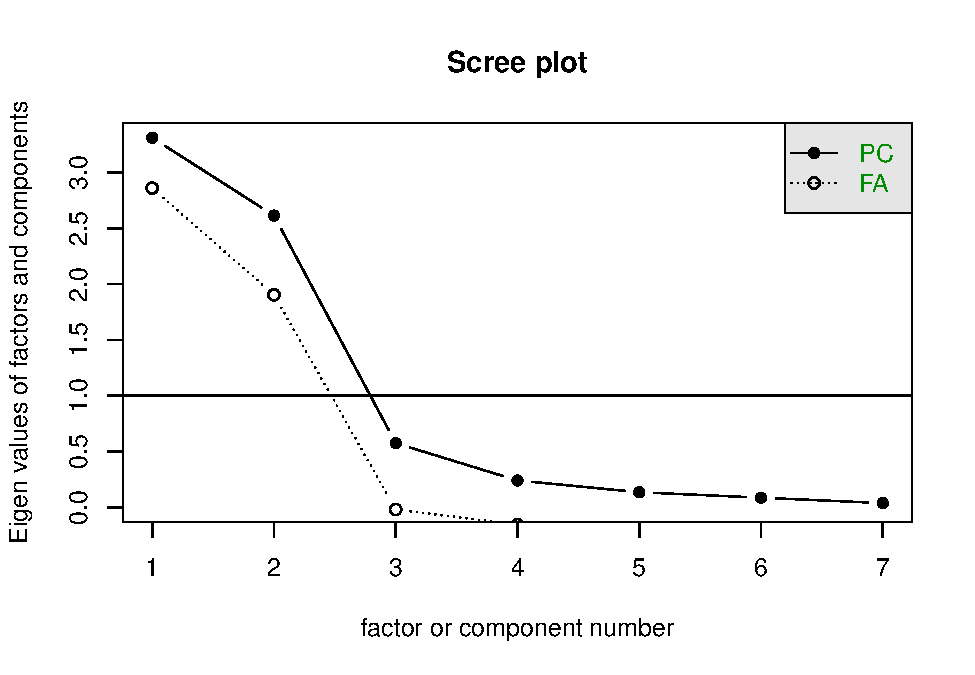
\includegraphics{timaglosur_files/figure-latex/skriduprof-1.pdf}
\caption{\label{fig:skriduprof}Skriðupróf bjórskala}
\end{figure}

\begin{itemize}
\tightlist
\item
  Samhliðagreining (parallel analysis)

  \begin{itemize}
  \tightlist
  \item
    Greining sem byggir á samanburði milli eigenvalues sem koma úr úrtaksgögnum með eigenvalues úr algjörlega random gögnum.
  \item
    Aðferðin byggir á þeirri hugmynd að m- stærstu eigenvalues úr reduced correlation matrix ætti að vera umtalsvert stærri heldur en m stærstu eigenvalues úr corresponding setti handahófskenndra gagna (handahófskennt gagnasafn með af sömu stærð og með sama fjölda mælibreyta).
  \item
    Viðeigandi fjöldi common þátta er fjöldi eigenvalues sem eru stærri en corresponding eigenvalues úr random gögnum.
  \end{itemize}
\end{itemize}

Skriðupróf fyrir PCA og þáttagreiningu má sjá í mynd \ref{fig:samhlidagreining}

\begin{figure}
\centering
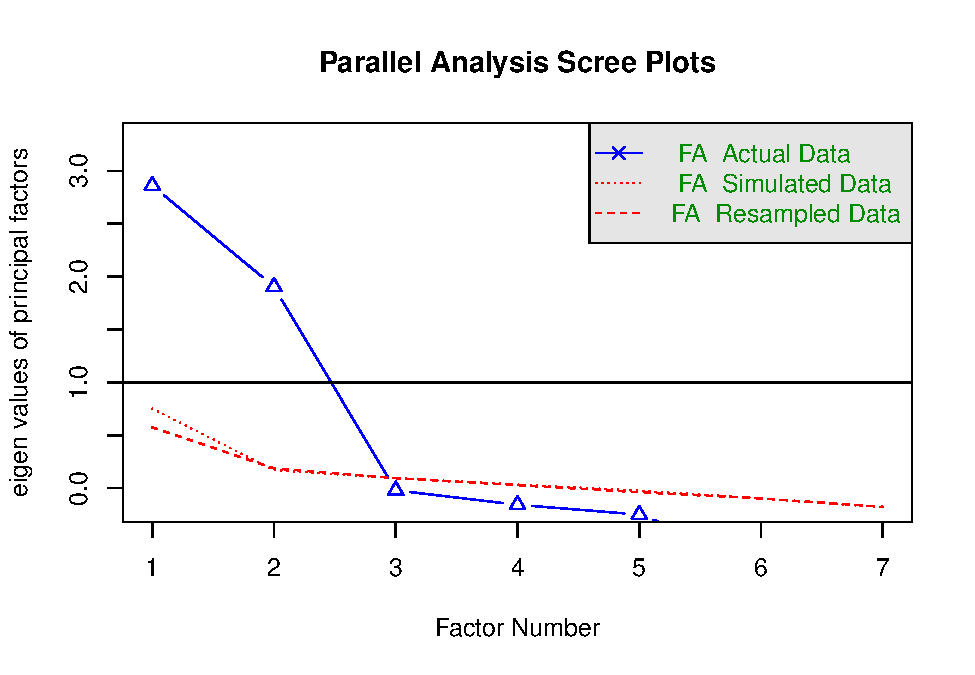
\includegraphics{timaglosur_files/figure-latex/samhlidagreining-1.pdf}
\caption{\label{fig:samhlidagreining}Samhliðagreining bjórskala}
\end{figure}

\begin{verbatim}
FALSE Parallel analysis suggests that the number of factors =  2  and the number of components =  NA
\end{verbatim}

\begin{itemize}
\tightlist
\item
  Likelihodd ratio test

  \begin{itemize}
  \tightlist
  \item
    Hægt að nota þegar um er að ræða ML
  \item
    Þá er hægt að reikna fleiri en eina þáttalausn, með mismörgum þáttum og kanna hver er með hæstu mátgæðin, samkvæmt kíkvaðrat.
  \item
    Hægt að vinna þessa umræðu lengra með því að búa til difference test (sem vill svo heppilega til að dreifist líka samkvæmt kí-kvaðrat) og þá er hægt að meta hvort fleiri eða færri þættir skili marktækri bætingu á mátgæðum.
  \end{itemize}
\item
  Model fit indices

  \begin{itemize}
  \tightlist
  \item
    Samskonar hugmynd hér að baki og við að nota likelihood ratio test
  \end{itemize}
\item
  Stability of solutions

  \begin{itemize}
  \tightlist
  \item
    Ef um er að ræða tvö eða fleiri gagnasöfn eða hægt er að skipta gagnasafni rannsóknarinnar í tvo eða fleiri hluta
  \item
    Þá er hægt að skoðu stöðugleika lausnarinnar yfir mismunandi gagnasöfn.
  \end{itemize}
\item
  Interpretability of solutions

  \begin{itemize}
  \tightlist
  \item
    Þáttagreining meikar bara sens ef hægt er að túlka endanlega þáttalausn
  \item
    Þannig að -- ef of margir eða of fáir þættir sem hamla túlkun þáttalausnarinnar þá er það til marks um að fleiri (eða færri) þættir ættu að vera dregnir út.
  \end{itemize}
\end{itemize}

\hypertarget{uxfeuxe1ttasnuxfaningur}{%
\section{Þáttasnúningur}\label{uxfeuxe1ttasnuxfaningur}}

\hypertarget{einfuxf6ld-formgeruxf0-simple-structure}{%
\subsection{Einföld formgerð (simple structure)}\label{einfuxf6ld-formgeruxf0-simple-structure}}

Helsta ástæða þess að nauðsynlegt er að snúa upprunalegu þáttalausninni er að einfalda túlkun og auka skýrleika þáttalausnarinnar. Mikilvægt er að hafa í huga að með snúningi þáttalausnarinnar er ekki verið að eiga við niðurstöðurnar, per se, heldur frekar að breyta því hvar undirliggjandi þættirnir lenda með tilliti til mældu breytanna. Það sem rannsakendur eru að leita eftir er það sem nefnt hefur verið einföld formgerð (simple structure) sem er safn einkenna á þáttalausn sem eru eftirsóknarverð. Í einfaldri formgerð koma fram þrenns konar almennir eiginleikar einfaldrar formgerðar:

\begin{itemize}
\tightlist
\item
  Á hvern þátt hlaða ákveðnar mældar breytur með háum hleðslum en aðrar breytur hafa lágar þáttahleðslur

  \begin{itemize}
  \tightlist
  \item
    Það er semsagt eftirsóknarvert að vera með sundurgreiningu hleðsla á þáttunum.
  \item
    Eðli málsins viltu að þær breytur sem eru með sterkustu tengslin við undirliggjandi þáttinn hafi háar hleðslur en aðrar mældar breytur hlaða veikar á þátinn
  \end{itemize}
\item
  Mældar breytur sem hlaða á mismunandi þætti ættu ekki að skarast nema að litlu leyti

  \begin{itemize}
  \tightlist
  \item
    Ekki er æskilegt að sömu breyturnar hlaði á alla þættina, sérstaklega ekki sterklega þar sem þá er sundurgreining þáttanna lítil sem engin.
  \end{itemize}
\item
  Hver mæld breyta æti aðeins að vera undir áhrifa frá hlutmengi þátta.

  \begin{itemize}
  \tightlist
  \item
    Það er, þú vilt ekki hafa þáttalausn þar sem allir þættir hlaða á allar mældar breytur.
  \end{itemize}
\end{itemize}

Upphaflega hugmyndin um einfalda formgerð kemur frá Thurstone (1947) og var hún þá sett fram sem fimm almennar leiðsagnarreglur:

\begin{enumerate}
\def\labelenumi{\arabic{enumi})}
\tightlist
\item
  Hver röð (það er, hver mæld breyta) í þátthleðslufylkinu á að innihalda að minnsta kosti eitt núll (eða gildi sem er mjög nálægt núlli).
\item
  Hver dálkur (það er, hver þáttur) ætti að innihalda að minnsta kosti m núll gildi -- eða m gildi sem eru mjög nálægt núlli (þar sem m er til marks um fjölda þátta í lausninni).
\item
  Hverjir tveir dálkar í þáttahleðslufylkinu (það er, hvert par þátta) ættu að hafa nokkrar raðir með núll eða gildum sem eru nærri núlli í einum dálknum en ekki í öðrum.
\item
  Í tilvikum þar sem m er fjórir eða meira, þá ætti hvert par dálka í þáttahleðslufylkinu að hafa nokkrar raðir með núlli eða gildi sem er nærri núlli í báðum dálkum.
\item
  Hvert par af dálkum í þáttahleðslufylkinu ætti að hafa aðeins fáar ráðir af hleðslum sem ekki eru núll í báðum dálkum.
\end{enumerate}

Ef um er að ræða þáttalausn sem uppfyllir vel þessi skilyrði þá er hún, miðað við aðrar mögulegar þáttalausnir:
- auðtúlkanlegri
- merkingarbærari hvað varðar hugsmíðirnar sem verið er að mæla
- líklegri til að koma ítrekað fram í frekari rannsóknum innan viðkomandi fræðasviðs

Þess vegna er það markmið rannsakenda (að mati Thurstones) að snúa ásum upphaflegu þáttalausnarinnar til að hámarka einfalda formgerð og byggja greiningu sína og túlkun á niðurstöðum þessarar snúnu lausnar.

Mikilvægt er að átta sig á því að leiðbeiningar Thurstones segja ekki að hver mæld breyta eigi aðeins að hlaða á einn þátt (sérstaklega þegar um er að að ræða þáttalausn með þremur eða fleiri þáttum). Það sem leiðsagnarreglur Thurstones segja hins vegar er að mæld breyta eigi ekki að hlaða á alla þættina. Í mörgum tilfellum er hægt að gera ráð fyrir að mæld breyta sé undir áhrifum fleiri en eins þáttar í þáttalausninni.

\begin{itemize}
\tightlist
\item
  Ef um er að ræða þáttalausn þar sem hver mæld breyta hleður aðeins á einn þátt þá nefnist það independent cluster solution. Slík lausn er sérstakt tilvik um einfalda formgerð en ekki eina tilvikið þar sem um er að ræða einfalda formgerð.
\end{itemize}

\hypertarget{uxfeegar-uxfeuxe1ttum-er-snuxfaiuxf0}{%
\subsection{Þegar þáttum er snúið}\label{uxfeegar-uxfeuxe1ttum-er-snuxfaiuxf0}}

Mikilvægt er að hafa hugfast að þegar þáttagreining er keurð þá eru til endalaust magn af jafngóðum lausnum fyrir niðurstöðurnar. Þess vegna er það nokkurn veginn undir hælinn lagt hvaða niðurstaða kemur fram þegar upprunalega þáttagreiningin er keyrð. Að minnsta kosti er ekkert sem passar upp á að niðurstöðurnar séu til marks um einfalda formgerð. Þess vegna beitum við snúningi á þáttalausnina, til að tryggja að lausnin sem við endum með einkennist af einfaldri formgerð.

\hypertarget{ruxfamfruxe6uxf0ileg-framsetning-uxfeuxe1ttagreiningar}{%
\subsubsection{Rúmfræðileg framsetning þáttagreiningar}\label{ruxfamfruxe6uxf0ileg-framsetning-uxfeuxe1ttagreiningar}}

Oft er þægilegra að skilja þáttagreiningu, og þá sérstaklega þáttasnúning, með því að setja líkanið fram á rúmfræðilegu formi (spatial representation). Þá er hægt að skoða niðurstöðurnar í tvívíðu rými þar sem þættirnir eru til marks um víddir eða ásana í rýminu og þáttahleðslurnar (aka vogtölurnar) eru til marks um hnit mældu breytanna í rýminu. Dæmi um þessa framsetningu má sjá í mynd \ref{fig:osnuinlausn} þar sem sjá má rúmfræðilega framsetningu á tveggja þátta lausn af ávarðanatöku bjórkaupenda. Í myndinni er um að ræða tvo þætti (sem ekki er búið að snúa) sem báðir tengjast því hvað skiptir neytendur máli þegar ákvörðun er tekinu um kaup á bjórkippu, annars vegar er það þátturinn hagkvæmni og hins vegar þátturinn bjórsnobb. Þegar myndir af þessu tagi eru túlkaðar er fjarlægðin milli mældu breytanna skoðuð. Þar sem um er að ræða háa, jákvæða fylgni milli breyta þá eru þær nærri hvor annarri. Þegar um er að ræða neikvæða fylgni þá er lengri fjarlægð milli breytanna í hnitakerfinu.

Eins og sjá má á myndinni mætti sjá fyrir sér að hægt væri að einfalda formgerðina með því að beita þáttasnúningi.

\begin{figure}
\centering
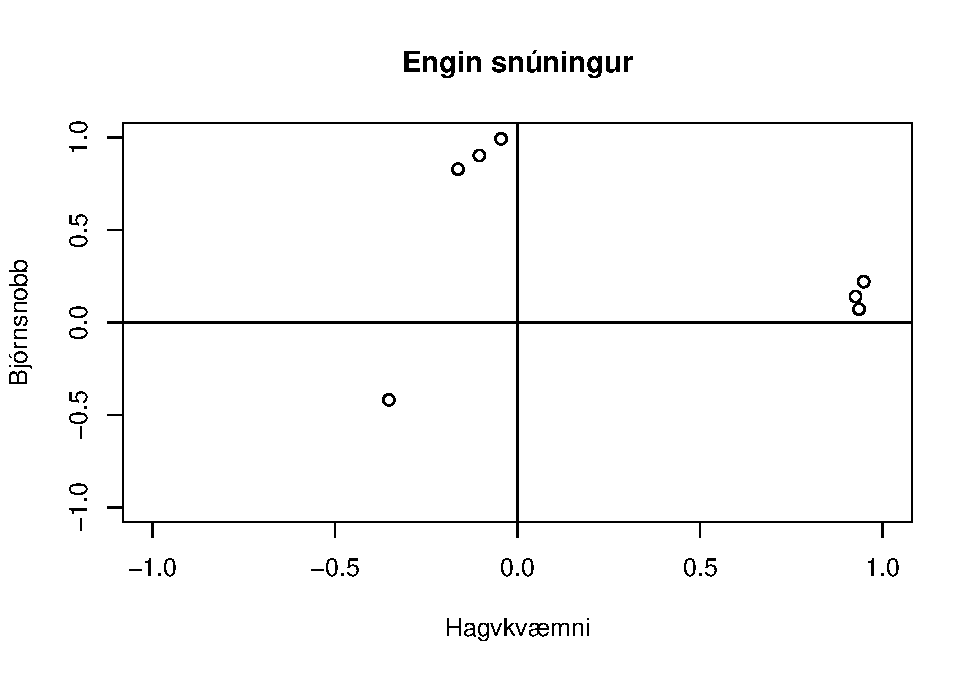
\includegraphics{timaglosur_files/figure-latex/osnuinlausn-1.pdf}
\caption{\label{fig:osnuinlausn}Ósnúin lausn}
\end{figure}

Mátgæði líkansins felast í því að hvaða marki rýmisleg fjarlægð milli mældu breytanna getur á nákvæman hátt endurgert (reconstruct) hina mældu fylgni milli mældu breytanna (observed correlations among measured variables). Ef þessi endurgerð er ónákvæm þá getur það kallað á flóknara líkan -- það er, að nota frekar þrjár víddir sem merkir þá að þriggja þátta líkan gæti virkað betur en tveggja þátta.

Mikilvægt atriði er að það hversu vel rýmisleg uppsetning getur gert grein fyrir mældri fylgni veltur ekki á nokkurn hátt á víddunum tveimur sem eru teiknaðar á myndinni. Það er, við getum snúið víddunum hvernig sem við viljum og sú framsetning myndi virka jafn vel til að skýra fylgnina. Snúningur víddanna myndi krefjast þess að ný hnit yrðu reiknuð (það er, þáttahleðslur) sem væru til marks um nýja staðsetningu víddanna (ásanna). En þessi hnit væru alveg jafngóð og hin fyrri við að skýra gögnin. Það er, snúningur víddanna myndi ekki breyta grundvallar fjarlægðinni í tvívíðu rúmi sem eru notaðar til að tákna og meta fylgni milli mældu breytanna.

Ein áskorun EFA er að ákvarða hvaða snúningur þáttanna er heppilegastur. Það er, hvaða lausn eigum við að velja úr þessum endalausa fjölda lausna sem allar passa jafn vel. Til að þáttagreining gangi upp eru í upphafi settar fram ákveðin skilyrði þannig að lausnin uppfylli tiltekin stærðfræðilegar forsendur. Þessar forsendur verða aðeins uppfylltar með ákveðnum snúningi lausnarinnar. Þessi lausn er aðeins valin til að hægt sé að ljúka þáttagreiningunni en mikilvægt er að valin verði lausn sem er til marks um einfalda formgerð.

\hypertarget{tegundir-snuxfaninga}{%
\subsubsection{Tegundir snúninga}\label{tegundir-snuxfaninga}}

Í fyrstu voru snúningar unnir í höndunum út frá myndrænni birtingu þáttalausnarinnar en í kringum 1950 voru rannsakendur byrjaðir að snúa þáttalausn með sjálfvirkum aðferðum. Slíkar aðferðir skiptast í tvennt: Hornréttan (orthogonal) og hornskakkan (oblique) snúning.

\textbf{Hornréttur snúningur} byggja á því að engin fylgni er leyfð milli þáttana þegar þeim er snúið. Í rúmfræðilegri lausn merkir þetta að passað sé upp á að hornið milli þáttanna þarf alltaf að vera 90°. Þaðan kemur nafnið. Dæmi um aðferðir sem falla undir yfirheitið hornskakkur þáttasnúningur eru:

\begin{itemize}
\tightlist
\item
  quartimax
\item
  varimax
\end{itemize}

Í mynd \ref{fig:hornrettlausn} má sjá þegar bjórkvarðanum hefur verið snúið með hornréttum Varimax snúningi. Eins og sjá má á myndinni þá skera ásar þáttanna betur í gegnum sett mældu breytanna heldur en þegar um var að ræða ósnúna þáttalausn.

\begin{figure}
\centering
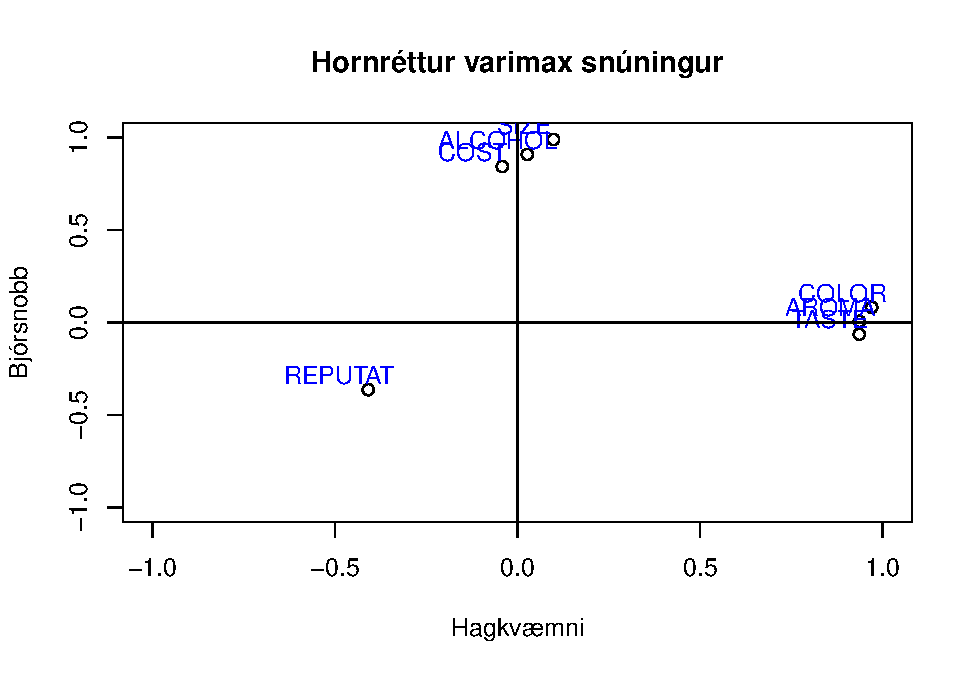
\includegraphics{timaglosur_files/figure-latex/hornrettlausn-1.pdf}
\caption{\label{fig:hornrettlausn}Snúin, hornrétt lausn}
\end{figure}

\textbf{Hornréttur snúningur} byggir á þeirri forsendu að fylgni milli þátta er leyfð. Oft þegar leitandi þáttagreiningu er beitt er tiltölulega sterkur fræðilegur grundvöllur fyrir því að fylgni milli þátta sé leyfði. Stundum er það meiraðsegja svo að rannsakendur hafa sérstakan fræðilegan áhuga á því að skoða sérstaklega fylgni milli þátta auk þess sem mynstur milli þeirra getur gefið mikilvægar upplýsingar um eðli þeirra, til dæmis að hvaða marki aðgreining milli mismunandi þátta er sterk eða veik.

Rétt eins og fyrir hornréttan snúning þá kemur nafngiftin fyrir hornskakkan snúning úr því að skoða þáttalausn í rúmfræðilegri framsetningu hennar, þegar fylgni er leyfð milli þátta þá er horninu milli þáttavíddanna leyft að vera hvasst eða gleitt, allt eftir því hvort um er að ræða mikla eða litla fylgni milli þáttanna. Þannig verður hornið hvassara (lægra en 90° og færist nær 0°) eftir því sem fylgnin milli þáttanna er meiri.

Meðal mismunandi tegunda hornskakkra snúninga eru:

\begin{itemize}
\tightlist
\item
  Promax
\item
  Harris-Kaiser/Orthoblique rotaion

  \begin{itemize}
  \tightlist
  \item
    Parameter -- HK power

    \begin{itemize}
    \tightlist
    \item
      HKP= 1, varimat
    \item
      HKP=0,5 = Oblique roation
    \item
      HKP = 0, oblique rotation sem leitar að independent cluster solution
    \end{itemize}
  \end{itemize}
\item
  Direct quartimin
\item
  Direct olibmin
\end{itemize}

Í mynd \ref{fig:hornskokklausn} má sjá þegar bjórkvarðanum hefur verið snúið með hornskökkum promax snúningi. Eins og sjá má á myndinni þá skera ásar þáttanna enn betur í gegnum sett mældu breytanna heldur en í fyrri tveimr lausnunum.

\begin{figure}
\centering
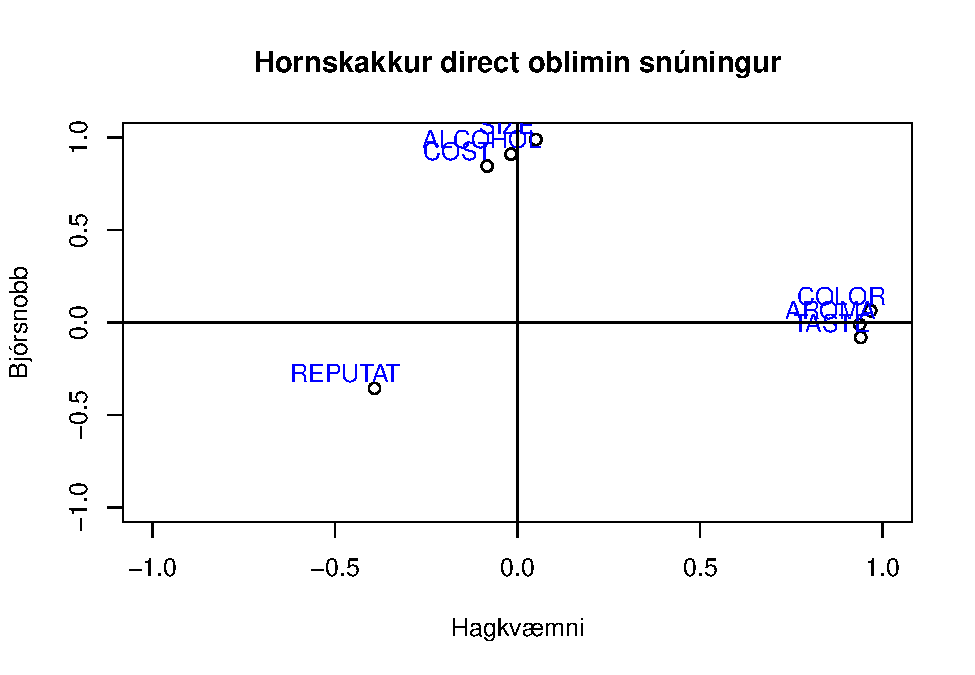
\includegraphics{timaglosur_files/figure-latex/hornskokkausn-1.pdf}
\caption{\label{fig:hornskokkausn}Snúin, hornskökk lausn}
\end{figure}

Til þess að glöggva okkur enn frekar á niðurstöðunum getum við skoðað hleðslur allra þriggja þáttalausnanna til að meta hver þessara þriggja lausna sé næst því að vera af einfaldari formgerð. Þetta má sjá fyrir þátt 1 sem kemur fram í töflu \ref{tab:samanbthatt1} og í töflu \ref{tab:samanbthatt2} fyrir þátt 2. Í þessu dæmi er sáralítill munur á hornskakkri og hornréttti þáttalausn og vart má á milli sjá hvor þeirra skilar einfaldari formgerð.

\begin{table}

\caption{\label{tab:samanbthatt1}Samanburður á þáttaleðslum þáttarins hagkvæmni í bjórkaupum fyrir ósnúna þáttalausn, hornrétta lausn og hornskakka lausn. }
\centering
\begin{tabular}[t]{l|r|r|r}
\hline
Breyta & Osnuin & Hornrett & Hornskokk\\
\hline
COST & -0.16 & -0.04 & -0.08\\
\hline
SIZE & -0.04 & 0.10 & 0.05\\
\hline
ALCHOLOL & -0.10 & 0.03 & -0.02\\
\hline
REPUTAT & -0.35 & -0.41 & -0.39\\
\hline
COLOR & 0.95 & 0.97 & 0.97\\
\hline
AROMA & 0.93 & 0.94 & 0.94\\
\hline
TASTE & 0.94 & 0.94 & 0.94\\
\hline
\end{tabular}
\end{table}

\begin{table}

\caption{\label{tab:samanbthatt2}Samanburður á þáttaleðslum þáttarins snobb í bjórkaupum fyrir ósnúna þáttalausn, hornrétta lausn og hornskakka lausn. }
\centering
\begin{tabular}[t]{l|l|r|r|r}
\hline
  & Breyta & Osnuin & Hornrett & Hornskokk\\
\hline
8 & COST & 0.83 & 0.84 & 0.85\\
\hline
9 & SIZE & 0.99 & 0.99 & 0.99\\
\hline
10 & ALCHOLOL & 0.90 & 0.91 & 0.91\\
\hline
11 & REPUTAT & -0.42 & -0.36 & -0.36\\
\hline
12 & COLOR & 0.22 & 0.08 & 0.06\\
\hline
13 & AROMA & 0.14 & 0.01 & -0.01\\
\hline
14 & TASTE & 0.07 & -0.06 & -0.08\\
\hline
\end{tabular}
\end{table}

\hypertarget{hornskakkur-euxf0a-hornruxe9ttur-snuxfaningur}{%
\subsubsection{Hornskakkur eða hornréttur snúningur?}\label{hornskakkur-euxf0a-hornruxe9ttur-snuxfaningur}}

Ákveðin hefð skapaðist fyrr á tímum fyrir að nota hornréttan snúning í leitandi þáttagreiningu en sú hefð varð að miklu leyti til vegna misskilnings. Ljóst er að hornskakkar aðfeðrir við þáttasnúning eru mun skynsamlegri. Helstu ástæður þess að hornréttur snúningur átti meiri vinsældum að fagna heldur en hornskakkur snúningur eru:

\begin{enumerate}
\def\labelenumi{\arabic{enumi})}
\item
  Af því að það tók langan tíma til að finna viðunandi hornskakkar snúningsaðferðir en hornréttar hafa lengi, lengi verið til. Þá getur verið að menn hafi einfaldlega verið að nota aðferð sem hafi verið notuð áður.
\item
  Ýmis konar misskilningur hefur valdið því að hornréttur snúningur væri heppilegri
\end{enumerate}

\begin{enumerate}
\def\labelenumi{\alph{enumi})}
\item
  Talið var að hornskakkur snúningur annað hvort krefðist þess að fylgni sé til staðar milli þáttanna eða valdi því að fylgni komi fram. Það er rangt -- hornskakkur snúningur leyfir einfaldlega að það sé fylgni til staðar. Hún er almennari aðferð til snúnings sem leyfir bæði tengda og ótengda þætti. Ef engin fylgni er til staðar, þá verða niðurstöður afar svipaðar hvort sem hornréttum eða hornskökkum snúningi var beitt.
\item
  Hugmyndir um að hornréttur snúningur sé á einhvern hátt einfaldari og þess vegna muni þær frekar leiða til einfaldrar formgerðar miðað við hornskakkan. Hins vegar er það andstæða rétt -- þegar undirliggjandi þættirnir hafa fylgni sín á milli þá mun hornskakkur snúningur frekar leiða til einfaldrar formgerðar. Þetta má sjá á mjög skýran hátt á bls. 76 í F\&W, mynd 3.4 og á blaðsíðu 77, mynd 3.5.
\item
  Ef rannsakendur telja að þættirnir eigi að vera ótengdir eða vill að þeir séu ótengdir þá muni hornréttur snúningur á einhvern hátt uppfylla þetta markmið. Hins vegar ef þættirnir eru raunverulega tengdir þá mun snúningur sem gengur út frá því að þeir séu ótengdir ekki breyta þessari staðreynd. \textbf{Forsendur líkana breyta ekki gögnunum!}
\end{enumerate}

``\ldots{}oblique rotation is generally a more sensible approach than orthogonal rotation. Oblique rotations will often be a more realistic representation of the data, will provide a solution that allows for easier interpretation, and will give the researcher additional information not available in orthogonal rotations (i.e.,the correlations among common factors). (Fabrigar og Wegener, 2012, bls. 78)''

\hypertarget{tuxfalkun-snuxfainnar-uxfeuxe1ttalausnar}{%
\subsubsection{Túlkun snúinnar þáttalausnar}\label{tuxfalkun-snuxfainnar-uxfeuxe1ttalausnar}}

\begin{enumerate}
\def\labelenumi{\arabic{enumi})}
\item
  Skölunarátt (scaling direction) á þáttum er arbitrary. Það skiptir semsagt ekki máli hvort um er að ræða jákvæðar eða neikvæðar hleðslur á þáttinn. Fyrir tiltekna þáttalausn þá er semsagt í lagi að snúa formerkjum þáttahleðsla fyrir allar þáttahleðslur í tilteknum dálki þáttahleðslufylkisins. Slíkt (af því gefnu að þær séu gerðar fyrir öll element í dálknum) hafa ekki áhrif á mátgæði líkansins eða communalities fyrir mældar breytur.
\item
  Röð þáttanna eftir snúning er jafnan arbitrary. Þrátt fyrir að röð þáttanna í upprunalegri lausn hafi ákveðna merkingu (sá þáttur sem skýrir mest af dreifingu mældu breytanna, þ.e. hefur hæsta eigenvalue) er dreginn út fyrstur og svo koll af kolli, þá er það ekki nauðsynlega svo eftir snúning.
\end{enumerate}

Munur milli hornréttrar og hornskakkrar lausnar:

\begin{enumerate}
\def\labelenumi{\arabic{enumi})}
\tightlist
\item
  Túlkun
\end{enumerate}

\begin{itemize}
\tightlist
\item
  Þáttahleðslur hornréttrar lausnar má túlka sem fylgni milli þáttarins og mældu breytunnar -- eru milli -1 og 1 og skýrða dreifni má reikna með því að setja hleðsluna í annað veldi.
\item
  Í hornskakkri lausn er ekki lengur um að ræða staðlaðan stuðul sem hægt er að túlka sem fylgni -- heldur eru hleðslurnar sambærilegar við standardized partial regression coefficients. Þær eru til marks um staðlaða breytingu í mældu breytunni þegar um er að ræða einnar einingar aukningu í þættinum þegar búið er að stjórna fyrir (partial out) áhrifum allra annarra þátta í líkaninu. Geta því verið utan marka -1 og 1 (þó það sé sjaldgæft) og ekki er hægt að setja þá í annað veldi.
\item
  Factor correlation matrix sýnir fylgni milli þátta og er því fí fylkið sem áður hefur verið talað um.
\end{itemize}

\begin{enumerate}
\def\labelenumi{\arabic{enumi})}
\setcounter{enumi}{1}
\tightlist
\item
  Töflur
\end{enumerate}

\begin{itemize}
\tightlist
\item
  Í hornréttum snúningi verður til ein tafla með snúnum þáttahleðslum.
\item
  Forrit sýna hins vegar oft þrjár töflur þegar hornskökkum snúningur hefur verið beitt: Pattern matrix, structure matrix og factor correlation matrix.

  \begin{itemize}
  \tightlist
  \item
    Pattern matrix: Lamda, það er, snúið fylki þáttahleðslna
  \item
    ``\ldots{}the pattern matrix should be the primary basis for interpreting factors. It is these values that are the actual parameter estimates of the factor loading matrix in the common factor model. (Fabrigar og Wegener, 2012, bls. 81).''
  \item
    Structure matrix: Zero order correlations milli þáttanna og mældra breyta (fylgni milli hvers þáttar og mældu breytanna án þess að stjórna fyrir áhrifa annarra þátta í líkaninu) Inniheldur ekki parameter estimates fyrir lambda né hefur þessum gildum verið snúið fyrir einfalda formgerð.
  \item
    factor correlation matrix er tafla þar sem fram koma fylgnistuðlar fyrir tengsl milli þáttanna í líkaninu.
  \end{itemize}
\end{itemize}

\hypertarget{nokkur-fleiri-oruxf0-um-forsendur-uxfeuxe1ttagreiningar}{%
\section{Nokkur fleiri orð um forsendur þáttagreiningar}\label{nokkur-fleiri-oruxf0-um-forsendur-uxfeuxe1ttagreiningar}}

\hypertarget{forsendur-sem-eru-undirliggjandi-uxfeuxe1ttaluxedkaninu-common-factor-model}{%
\subsection{Forsendur sem eru undirliggjandi þáttalíkaninu (common factor model)}\label{forsendur-sem-eru-undirliggjandi-uxfeuxe1ttaluxedkaninu-common-factor-model}}

\hypertarget{effects-indicators-vs.causal-indicators}{%
\subsubsection{Effects indicators vs.~causal indicators}\label{effects-indicators-vs.causal-indicators}}

Í þáttagreiningu er gert ráð fyrir að skor á hverri mældri breytu í safni mældra breyta komi til vegna áhrifa undirliggjandi þáttar (common factor) og vegna áhrifa sem aðeins hafa áhrif á viðkomandi breytu (unique factor). Gert er ráð fyrir að þættirnir hafi línuleg orsakaáhrif á mældar breytur - \textgreater{} effects indicator models. Mældar breytur eru semsagt indicatorar fyrir undirliggjandi þættir -- þær eru áhrif þeirra.

Þetta meikar fullkomið sens fyrir ákveðnar breytur, eins og viðhorfamælingar, mælingar á greind og persónuleikamælingar. Hins vegar meikar þetta ekkert sens fyrir ýmsar aðrar mælingar og því kann að vera skynsamlegra (conceptually) að setja fram orsakasamband í hina áttina -\textgreater{} causal indicators models -- það er, mældu breyturnar eru orsakavaldar hinna undirliggjandi vídda. Dæmi úr bókinni er SES, sem er oft metið með því að sameina ýmsar mælingar á borð við menntun, occupational prestige og innkomu. Eins og gefur að skilja er það óskiljanlegt að setja það fram svoleiðis að SES valdi því hvernig viðkomandi hefur menntað sig, tekjur hans og starf.

Causal indicator models byggja ekki á því að mældar breytur í batteríi ættu að hafa háa innbyrðis fylgni. Módel af þessu tagi leyfa jafnan indicatorum að hafa innbyrðis fylgni en indicatorarnir sjálfir ættu aðeins að hafa fylgni innbyrðis að því marki sem þeir deila common antecedents. Þar sem engir antacedents eru tilgreindir í líkaninu þá er sá möguleiki opinn að indicatorarnir hafi fáa, ef einhverja sameiginlega antecedents.

EFA á aðeins við þar sem um er að ræða effects indicator model -- það er, þar sem rannsakandi getur gengið út frá því að slíkt líkan haldi. Þess vegna þarf alltaf, áður en ráðist er í að framkvæma EFA, að ákvarða hversu sennilegt það er að effects indicator model sé til staðar í rannsókninni sem viðkomandi stendur fyrir.

``If the sorts of constructs that are expected can be reasonably postulated to cause scores on measured variables, then EFA might well be a viable method of analysis. On the other hand, if a causal indicator model is more plausible, EFA should not be used. At the empirical level, there are really no clear exploratory methods for researchers to gauge the plausibility of their assumption of an eff ects indicator model in the context of EFA (although tests have been proposed for confirmatory latent variable models, see Bollen \& Ting, 2000). Strong correlations among all measured variables or subsets of measured variables within a battery are certainly consistent with an eff ects indicator model. However, as noted, causal indicator models do not preclude high correlations among measured variables. (pp.~92)''

\hypertarget{luxednuleg-euxf0a-uxf3luxednuleg-uxe1hrif-uxfeuxe1tta}{%
\subsubsection{Línuleg eða ólínuleg áhrif þátta}\label{luxednuleg-euxf0a-uxf3luxednuleg-uxe1hrif-uxfeuxe1tta}}

Önnur lykilforsenda þáttagreiningar er að þættirnir hafi línuleg áhrif á mældar breytur -\textgreater{} mældar breytur eru til marks um vigtaða línulega sameiningu þáttanna sem eru undirliggjandi öllum mælibreytunum og unique factor.

Þetta er algeng forsenda í aðferðum sem beitt er í félagsvísindum og sálfræði og oftast gengur hún upp. En ekki alltaf. Greinilegasta dæmið um það þegar breytur hafa verið mældar á nafn eða raðkvarða. Þáttahleðsla segir til um hallatölu aukningar (eða minnkunar þegar formerkið er mínus) í mælieiningu mældu breytunnar fyrir einnar einingar aukningu á þættinum. Þetta samband meikar aðeins sens ef gildi mældu breytunnar eru í röð og bilið á milli gildanna er jafnstórt hvar sem maður er staddur á kvarða breytunnar. Þess vegna skal aðeins beita þáttagreiningu þegar um er að ræða interval eða quasi-interval mælingum.

Það er hægt að þáttagreina tvíkosta breytur en slíkt skilar oft niðurstöðum sem eru misleading. Fyrst og fremst er það vegna þess að slík atriði skila oft erfiðleikaþáttum sem eru til marks um endorsement rate mældra breyta frekar en undirliggjandi hugsmíðar sem er verið að meta með mældu breytunum. Þess vegna er best að nota sérhæfðar þáttagreiningarlausnir þegar unnið er með tvíkostabreytur.

Stundum er ekki hægt að ganga út frá línulegum áhrif þáttarins á mældu breyturnar -- en það er þá alveg eins og í regression: Samvirkni eða sveiglínutengsl.

\hypertarget{forsendur-um-auxf0geruxf0ir-til-auxf0-fitta-luxedkani}{%
\subsubsection{Forsendur um aðgerðir til að fitta líkani}\label{forsendur-um-auxf0geruxf0ir-til-auxf0-fitta-luxedkani}}

Fjölbreytu normaldreifing er forsenda þegar ML er notað. Rannsóknir hafa hins vegar bent til þess að ML sé í lagi að því marki að ekki sé um að ræða alvarleg brot á forsendum, það er, ML þáttagreining er tiltölulega ónæm fyrir brotum á forsendum. En það er þó ekki þannig að hægt sé að líta fram hjá þessari forsendu og rannsakendum ber alltaf að taka hana með í reikninginn.

Af þessu vakna tvær spurningar:

\begin{enumerate}
\def\labelenumi{\arabic{enumi})}
\tightlist
\item
  Hvenær veit rannsakandi að frávik frá normaldreifingu séu nógu mikil til að bjaga niðurstöður að einhverju marki?
\item
  Ef um er að ræða alvarleg frávik frá forsendum, hvað er hægt að taka til bragðs?
\end{enumerate}

``Substantial distortions in ML parameter estimates did not emerge until measured variables had an absolute value of skew of two or greater and an absolute value of kurtosis of seven or greater. Thus, data sets with skew and kurtosis values substantially smaller than these guidelines are unlikely to present problems for ML EFA, whereas data sets at or above these values might be problematic. pp.~99''

Svo er að sjálfsögðu alltaf góð hugmynd að skoða vel og vandlega normalplot í gegnum hugbúnaðinn sem á að nota fyrir greininguna.

Hvað er hægt að gera?

\begin{enumerate}
\def\labelenumi{\arabic{enumi})}
\item
  Búa til parcels (aggregera saman nokkrar breytur í eina),
\item
  Nonlinear transformation, til dæmis power transformation. Log eða setja í annað veld. Box-Cox.,
\item
  Nota annars konar aðferð við að fitta módelinu og sleppa því að nota ML. Það er þó ekki mælt með þessu en hins vegar er hægt að skoða hvort aðrar aðferðir (sem ekki gera ráð fyrir multivariable normality) gefi allt aðrar niðurstöður heldur en aðferðir á borð við ML sem gera ráð fyrir normality. Með því fær rannsakandi betri hugmynd um það hvort dreifing breytanna hafi óæskileg áhrif á niðurstöður EFA.
\end{enumerate}

\hypertarget{fullkomin-luxednuleg-dependency-milli-muxe6ldra-breyta}{%
\subsubsection{Fullkomin línuleg dependency milli mældra breyta}\label{fullkomin-luxednuleg-dependency-milli-muxe6ldra-breyta}}

Annar eiginleiki mældra breyta er að engin mæld breyta í spurningalista (battery) sé fullkomin línuleg function af öðrum mældum breytum í batteríinu. Það er, ákveðin mæld breyta ætti ekki að vera accounted for af línulegri combination annarra mældra breyta eða línulegri transformation annarra mældra breyta í batteríinu. Þetta gæti til dæmis gerst ef rannsakandinn væri með mælda breyta í gagnasafninu sem væri summa eða meðaltal nokkrra annarra breyta í settinu. Þessi aggregeraða breyta væri fullkomlega skýrt af mældum breytunum sem voru notaðar til að reikna hana.

Þetta leiðir til villu - \textgreater{} not positive definite.

\bibliography{book.bib,packages.bib}


\end{document}
